\documentclass{article}%
\usepackage[T1]{fontenc}%
\usepackage[utf8]{inputenc}%
\usepackage{lmodern}%
\usepackage{textcomp}%
\usepackage{lastpage}%
%
\usepackage{amsmath}%
\usepackage{amssymb}%
\usepackage{amsfonts}%
\usepackage{graphicx}%
\usepackage{hyperref}%
\usepackage{tikz}%
\usepackage{pgfplots}%
\usetikzlibrary{math}%
\title{IME 2026 - Química\thanks{This exam was solved and automatically generated with gpt-resolve: \url{https://github.com/lgabs/gpt-resolve}}}%
\author{claude{-}sonnet{-}5{-}5 (solver) + claude{-}sonnet{-}5{-}5 (judge)}%
\date{November 10, 2026}%
%
\begin{document}%
\normalsize%
\maketitle%
\section*{Questão 1}

\section*{Solução}

\textbf{1. Modelo e hipóteses.} Na eletrólise ígnea do $\text{MC}\ell_2$ (sal fundido, sem água) existem apenas os íons $\text{M}^{2+}$ e $\text{C}\ell^-$. A própria fórmula $\text{MC}\ell_2$ fixa a carga do cátion em $+2$, logo $z=2$.
\[
\text{Cátodo (redução): } \text{M}^{2+} + 2\,e^- \longrightarrow \text{M}(s), \qquad
\text{Ânodo (oxidação): } 2\,\text{C}\ell^- \longrightarrow \text{C}\ell_2(g) + 2\,e^-.
\]
Hipóteses: corrente constante e rendimento de $100\%$, isto é, a única reação catódica é a deposição de M. Isso é razoável porque não há água no sistema. Em meio aquoso, um metal de potencial de redução muito negativo não se depositaria, pois a água seria reduzida antes. É por isso que o enunciado exige o sal fundido. Vale a 1ª lei de Faraday: a massa depositada é proporcional à carga que atravessa o circuito.

\textbf{2. Carga elétrica.} $t = 6{,}7\ \text{h} = 6{,}7\times 3600 = 24120\ \text{s}$, logo
\[
Q = i\,t = 0{,}4\times 24120 = 9648\ \text{C}.
\]

\textbf{3. Quantidade de elétrons.} Com $F = 96480\ \text{C}\cdot\text{mol}^{-1}$ (folha de dados),
\[
n_{e^-} = \frac{Q}{F} = \frac{9648}{96480} = 0{,}100\ \text{mol}.
\]

\textbf{4. Quantidade de metal.} Na semirreação catódica, $2$ mol de elétrons depositam $1$ mol de M:
\[
n_\text{M} = \frac{n_{e^-}}{z} = \frac{0{,}100}{2} = 0{,}050\ \text{mol}.
\]

\textbf{5. Massa molar.}
\[
M_\text{M} = \frac{m}{n_\text{M}} = \frac{4{,}38\ \text{g}}{0{,}050\ \text{mol}} = 87{,}6\ \text{g}\cdot\text{mol}^{-1}.
\]

\textbf{6. Identificação.} Um metal que forma o cátion $\text{M}^{2+}$ e tem massa atômica $\approx 87{,}6$ está na região do $5^\circ$ período, entre o Rb ($85{,}47$) e o Y ($88{,}91$). O único elemento da Tabela Periódica com massa atômica compatível é o estrôncio, $\text{Sr}$ ($Z=38$, $87{,}62$). Ele é do grupo 2 (alcalinoterroso), forma $\text{Sr}^{2+}$ e o sal $\text{SrC}\ell_2$, o que concorda com a fórmula do enunciado. Seu potencial de redução, $E^\circ(\text{Sr}^{2+}/\text{Sr})\approx -2{,}9\ \text{V}$, explica por que ele só pode ser obtido por eletrólise ígnea.

\textbf{7. Verificações.}
\begin{itemize}
\item \emph{Conferência inversa:} $0{,}050\ \text{mol}\times 87{,}62\ \text{g}\cdot\text{mol}^{-1} = 4{,}381\ \text{g}\approx 4{,}38\ \text{g}$.
\item \emph{Sensibilidade a $F$:} com $F=96500\ \text{C}\cdot\text{mol}^{-1}$ obtém-se $87{,}62\ \text{g}\cdot\text{mol}^{-1}$. O resultado praticamente não muda.
\item \emph{Incerteza.} Os dados do enunciado são numericamente ``redondos'': $Q = 9648\ \text{C} = 0{,}1000\,F$ exatamente. Por isso foram tratados como valores nominais exatos, e o resultado $87{,}6$ vem de $m$ com três algarismos significativos ($87{,}5$ a $87{,}7$). Se $t = 6{,}7 \pm 0{,}05\ \text{h}$ for tomado como incerteza de leitura, junto com $m = 4{,}38 \pm 0{,}005\ \text{g}$, a incerteza propagada é de cerca de $\pm 0{,}7\ \text{g}\cdot\text{mol}^{-1}$. Mesmo assim, Y (diferença $\approx 1{,}3$) e Rb (diferença $\approx 2{,}1$) continuam excluídos. Rb ainda é monovalente e Y é trivalente, incompatíveis com $\text{MC}\ell_2$. A incerteza de $i$ não foi incluída, pois só um valor nominal exato permite identificar o elemento.
\item \emph{Valência:} a fórmula $\text{MC}\ell_2$ impõe $z=2$. Um $z$ diferente ($1$ ou $3$) daria $43{,}8$ ou $131{,}4\ \text{g}\cdot\text{mol}^{-1}$, valores incompatíveis com um metal que forme $\text{MC}\ell_2$.
\item \emph{Unidades:} $\text{A}\cdot\text{s}=\text{C}$; $\text{C}/(\text{C}\cdot\text{mol}^{-1})=\text{mol}$; $\text{g}/\text{mol}$ é unidade de massa molar.
\item \emph{Ordem de grandeza:} $0{,}4\ \text{A}$ durante $\approx 7\ \text{h}$ transporta $\approx 10^{4}\ \text{C}$, isto é, $\approx 0{,}1$ mol de elétrons. Isso deposita $\approx 0{,}05$ mol de um metal divalente, ou seja, alguns gramas, compatível com $4{,}38$ g.
\end{itemize}

O metal M é o \textbf{estrôncio (Sr)}.

ANSWER: M = estrôncio (Sr), $Z = 38$, com massa molar $\approx 87{,}6\ \text{g}\cdot\text{mol}^{-1}$.%
\newpage%
\section*{Questão 2}

\section*{Solução}

\textbf{Passo 0 --- Fórmulas e insaturações.}
$\mathrm{C_5H_{11}C\ell}$ tem grau de insaturação $\frac{2\cdot 5+2-11-1}{2}=0$: A é um cloreto de alquila saturado e acíclico. A desidro-halogenação (eliminação de $\mathrm{HC\ell}$, base forte/álcool) forma B $=\mathrm{C_5H_{10}}$, com uma insaturação, isto é, um \textbf{alceno}. A hidratação de B dá C $=\mathrm{C_5H_{12}O}$.

\textbf{Passo 1 --- Ozonólise: B é um alceno terminal.}
Na ozonólise com tratamento redutivo ($\mathrm{O_3}$; depois $\mathrm{Zn/H_2O}$), cada carbono da dupla vira $\mathrm{C{=}O}$. Com tratamento oxidativo, o formaldeído seria oxidado a $\mathrm{HCOOH}$ ou $\mathrm{CO_2}$, por isso se entende que é redutivo. O formaldeído $\mathrm{H_2C{=}O}$ só se origina de um grupo $\mathrm{=CH_2}$, logo B é um \emph{1-eno}. Os alcenos sem $\mathrm{=CH_2}$ ficam excluídos: pent-2-eno (etanal + propanal) e 2-metilbut-2-eno (propanona + etanal). Restam três candidatos:
\[
\text{pent-1-eno},\qquad \text{2-metilbut-1-eno},\qquad \text{3-metilbut-1-eno}.
\]

\textbf{Passo 2 --- Hidratação: C é álcool terciário.}
A hidratação ácida ($\mathrm{H_2O/H^+}$) segue Markovnikov: o $\mathrm{OH}$ entra no carbono mais substituído da dupla, via carbocátion. A hidroboração-oxidação (anti-Markovnikov) daria álcool primário, e não é a reação do enunciado. O $\mathrm{KMnO_4/H^+}$ oxida álcoois primários (a ácido carboxílico) e secundários (a cetona), porque o carbono carbinólico tem H. Um álcool \textbf{terciário} não tem esse H e não é oxidado. Logo, C é álcool terciário (item a).

\begin{itemize}
\item pent-1-eno $\to$ cátion secundário $\to$ pentan-2-ol (secundário). O deslocamento de H só leva a outro cátion secundário (pentan-3-ol). \emph{Não serve.}
\item 2-metilbut-1-eno $\to$ cátion terciário $\mathrm{(CH_3)_2C^+CH_2CH_3}$ $\to$ $\mathrm{(CH_3)_2C(OH)CH_2CH_3}$, 2-metilbutan-2-ol (terciário). \emph{Serve.}
\item 3-metilbut-1-eno: a adição direta de Markovnikov dá o cátion secundário e o 3-metilbutan-2-ol (secundário, oxidável). Em meio ácido, porém, esse cátion pode sofrer \emph{migração de hidreto 1,2} para o cátion terciário $\mathrm{(CH_3)_2C^+CH_2CH_3}$ e levar ao \emph{mesmo} 2-metilbutan-2-ol. Portanto, a rigor, ele também seria compatível com C.
\end{itemize}
O enunciado pede uma estrutura única para B. Adota-se o critério de Markovnikov sem rearranjo, que é o caminho direto. Ele dá B $=$ 2-metilbut-1-eno, cujo carbocátion já é terciário. De qualquer modo, \textbf{C é o mesmo} nos dois casos e o item (a) não depende dessa escolha:
\[
\mathrm{CH_2{=}C(CH_3)CH_2CH_3 + H_2O \xrightarrow{\;H^+\;} (CH_3)_2C(OH)CH_2CH_3}\quad(\text{C}).
\]

\textbf{Conferência da ozonólise de B:}
\[
\mathrm{CH_2{=}C(CH_3)CH_2CH_3 \xrightarrow{\;1)\,O_3;\ 2)\,Zn/H_2O\;} H_2C{=}O + CH_3C(=O)CH_2CH_3}
\]
Formam-se formaldeído e butanona, como exigido.

\textbf{Passo 3 --- Estrutura de A.}
A é um cloreto de alquila $\mathrm{C_5H_{11}C\ell}$ com o esqueleto do 2-metilbutano que, por eliminação de $\mathrm{HC\ell}$, forma a dupla $\mathrm{C1{=}C2}$. A escolha mais coerente é pôr o Cl em C1, de modo que o único carbono $\beta$ seja C2:
\[
\mathrm{C\ell CH_2{-}CH(CH_3){-}CH_2CH_3 \xrightarrow{\;\text{KOH/álcool},\ \Delta\;} CH_2{=}C(CH_3)CH_2CH_3 + HC\ell}
\]
O A é o \textbf{1-cloro-2-metilbutano}. Como C1 tem um único carbono $\beta$, B é o único alceno formado, sem mistura.

\textbf{Observação sobre A.} O 2-cloro-2-metilbutano também leva a B, mas só como produto minoritário. Com base pequena (etóxido, regra de Zaitsev), o produto principal seria o 2-metilbut-2-eno, que dá propanona e etanal na ozonólise, sem formaldeído. Com base volumosa (\emph{terc}-butóxido, regra de Hofmann), B passa a ser majoritário. Esse isômero é, portanto, uma resposta alternativa aceitável sob essa condição. O 1-cloro-2-metilbutano é a opção que gera B sem depender do tipo de base.

\textbf{Respostas.}

a) C é um \textbf{álcool terciário}. O carbono que leva o $\mathrm{OH}$ não tem hidrogênio, então C não é oxidado por $\mathrm{KMnO_4/H^+}$.

b)
\begin{align*}
\text{A} &: \mathrm{C\ell CH_2{-}CH(CH_3){-}CH_2{-}CH_3}\ \text{(1-cloro-2-metilbutano)},\\
\text{B} &: \mathrm{CH_2{=}C(CH_3){-}CH_2{-}CH_3}\ \text{(2-metilbut-1-eno)},\\
\text{C} &: \mathrm{(CH_3)_2C(OH){-}CH_2{-}CH_3}\ \text{(2-metilbutan-2-ol)}.
\end{align*}

ANSWER: a) álcool (terciário). b) A = 1-cloro-2-metilbutano, $\mathrm{C\ell CH_2CH(CH_3)CH_2CH_3}$ (alternativa: 2-cloro-2-metilbutano com base volumosa); B = 2-metilbut-1-eno, $\mathrm{CH_2{=}C(CH_3)CH_2CH_3}$; C = 2-metilbutan-2-ol, $\mathrm{(CH_3)_2C(OH)CH_2CH_3}$.%
\newpage%
\section*{Questão 3}

\section*{Solução}

\textbf{Fórmula molecular.} A razão C:H:O $=6:10:1$ com dois átomos de oxigênio (i) dá $\mathrm{C_{12}H_{20}O_2}$ (massa molar $\approx 196\ \mathrm{g\cdot mol^{-1}}$). O índice de insaturação é $(2\cdot 12+2-20)/2=3$: duas ligações $\mathrm{C{=}C}$ (dieno) e uma $\mathrm{C{=}O}$ (éster), coerente com um acetato (éster do ácido acético com o álcool linalol).

\textbf{a) Montagem da estrutura.}
\begin{enumerate}
\item (ii) e (iii): cadeia principal de 8 C numerada a partir da extremidade com a dupla $\mathrm{C1{=}C2}$; a outra dupla é $\mathrm{C6{=}C7}$. Entre as duplas ficam $\mathrm{C3,C4,C5}$ (três carbonos), logo o dieno é \emph{não conjugado} (1,6).
\item (iv): duas metilas na mesma extremidade: $\mathrm{C8}$ (fim da cadeia) e uma metila ramificada em $\mathrm{C7}$, formando $\mathrm{=C(CH_3)_2}$.
\item Contagem: $12-8=4$ carbonos fora da cadeia principal: 2 do grupo acetato $\mathrm{(-O-CO-CH_3)}$ e 2 metilas (uma em $\mathrm{C7}$ e outra a localizar). Os dois O ficam no acetato.
\item (v): carbonos alílicos não terminais são $\mathrm{C3}$ (vizinho de $\mathrm{C2}$) e $\mathrm{C5}$ (vizinho de $\mathrm{C6}$). O $\mathrm{C5}$ está ao lado da dupla trissubstituída $\mathrm{C6{=}C7}$ (mais congestionada); o $\mathrm{C3}$ está ao lado da vinila monossubstituída, de menor impedimento. Logo a metila e o acetato estão em $\mathrm{C3}$.
\end{enumerate}

Fórmula estrutural plana (nome: acetato de 3,7-dimetilocta-1,6-dien-3-ila):

\begin{center}
\begin{tikzpicture}[x=1cm,y=1cm,font=\small,every node/.style={inner sep=1.5pt}]
\node (c1) at (0,0) {$\mathrm{H_2C}$};
\node (c2) at (1.6,0) {$\mathrm{CH}$};
\node (c3) at (3.2,0) {$\mathrm{C}$};
\node (c4) at (4.8,0) {$\mathrm{CH_2}$};
\node (c5) at (6.4,0) {$\mathrm{CH_2}$};
\node (c6) at (8.0,0) {$\mathrm{CH}$};
\node (c7) at (9.6,0) {$\mathrm{C}$};
\node (c8) at (11.2,0) {$\mathrm{CH_3}$};
\node (m3) at (3.2,1.4) {$\mathrm{CH_3}$};
\node (m7) at (9.6,1.4) {$\mathrm{CH_3}$};
\node (o)  at (3.2,-1.4) {$\mathrm{O}$};
\node (c)  at (3.2,-2.8) {$\mathrm{C}$};
\node (od) at (4.8,-2.8) {$\mathrm{O}$};
\node (me) at (1.6,-2.8) {$\mathrm{CH_3}$};
\draw (c2) -- (c3) -- (c4) -- (c5) -- (c6);
\draw (c7) -- (c8);
\draw ([yshift=1.6pt]c1.east) -- ([yshift=1.6pt]c2.west);
\draw ([yshift=-1.6pt]c1.east) -- ([yshift=-1.6pt]c2.west);
\draw ([yshift=1.6pt]c6.east) -- ([yshift=1.6pt]c7.west);
\draw ([yshift=-1.6pt]c6.east) -- ([yshift=-1.6pt]c7.west);
\draw (c3) -- (m3);
\draw (c7) -- (m7);
\draw (c3) -- (o) -- (c) -- (me);
\draw ([yshift=1.6pt]c.east) -- ([yshift=1.6pt]od.west);
\draw ([yshift=-1.6pt]c.east) -- ([yshift=-1.6pt]od.west);
\node[font=\scriptsize,gray] at (0,-0.55) {C1};
\node[font=\scriptsize,gray] at (1.6,-0.55) {C2};
\node[font=\scriptsize,gray] at (3.75,0.3) {C3};
\node[font=\scriptsize,gray] at (4.8,-0.55) {C4};
\node[font=\scriptsize,gray] at (6.4,-0.55) {C5};
\node[font=\scriptsize,gray] at (8.0,-0.55) {C6};
\node[font=\scriptsize,gray] at (10.15,0.3) {C7};
\node[font=\scriptsize,gray] at (11.2,-0.55) {C8};
\end{tikzpicture}
\end{center}

Forma condensada:
\[
\mathrm{CH_2{=}CH{-}C(CH_3)(OCOCH_3){-}CH_2{-}CH_2{-}CH{=}C(CH_3)_2}
\]
Conferência: $\mathrm{C}=12$ e $\mathrm{H}=2+1+3+3+2+2+1+6=20$.

\textbf{b) Poliadição na dupla mais substituída.} A dupla $\mathrm{C6{=}C7}$ é trissubstituída (três grupos alquila), enquanto $\mathrm{C1{=}C2}$ é monossubstituída; logo a poliadição ocorre em $\mathrm{C6{=}C7}$. Na adição, a ligação $\pi$ se abre e cada monômero passa a fazer duas ligações $\sigma$ $\mathrm{C{-}C}$ na cadeia principal, sem perda de átomos (a unidade repetitiva tem a mesma fórmula do monômero, $\mathrm{C_{12}H_{20}O_2}$). A dupla $\mathrm{C1{=}C2}$ (vinila) e o grupo acetato permanecem como ramificações laterais, com $\mathrm{R=-CH_2CH_2-C(CH_3)(OCOCH_3)-CH{=}CH_2}$.

\begin{center}
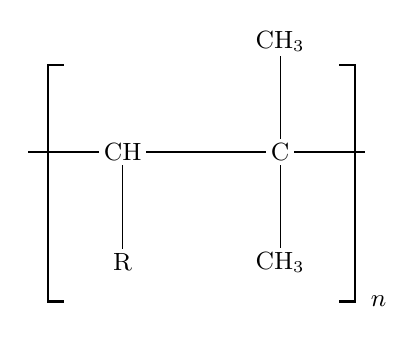
\begin{tikzpicture}[x=1cm,y=1cm,font=\small,every node/.style={inner sep=1.5pt}]
\node (a) at (0,0) {$\mathrm{CH}$};
\node (b) at (2,0) {$\mathrm{C}$};
\node (r) at (0,-1.4) {$\mathrm{R}$};
\node (m1) at (2,1.4) {$\mathrm{CH_3}$};
\node (m2) at (2,-1.4) {$\mathrm{CH_3}$};
\draw (a) -- (b);
\draw (a) -- (r);
\draw (b) -- (m1);
\draw (b) -- (m2);
\draw (a.west) -- ++(-0.9,0);
\draw (b.east) -- ++(0.9,0);
\draw[thick] (-0.75,1.1) -- (-0.95,1.1) -- (-0.95,-1.9) -- (-0.75,-1.9);
\draw[thick] (2.75,1.1) -- (2.95,1.1) -- (2.95,-1.9) -- (2.75,-1.9);
\node at (3.25,-1.9) {$n$};
\end{tikzpicture}
\end{center}

Em forma linear: $\left[-\mathrm{CH(R)-C(CH_3)_2-}\right]_n$.

Observações: (1) por ser terciário, o carbono $\mathrm{C7}$ estabiliza um carbocátion, o que favorece a iniciação catiônica nessa dupla; (2) as vinilas pendentes continuam insaturadas e permitem reações posteriores (por exemplo, reticulação). O enunciado pede o polímero ``possivelmente formado'', pois a dupla trissubstituída é estericamente impedida e polimeriza com dificuldade na prática.

\medskip
ANSWER: a) $\mathrm{CH_2{=}CH{-}C(CH_3)(OCOCH_3){-}CH_2{-}CH_2{-}CH{=}C(CH_3)_2}$ (acetato de 3,7-dimetilocta-1,6-dien-3-ila, $\mathrm{C_{12}H_{20}O_2}$); b) $\left[-\mathrm{CH(R)-C(CH_3)_2-}\right]_n$ com $\mathrm{R=-CH_2CH_2C(CH_3)(OCOCH_3)CH{=}CH_2}$ (vinila e acetato pendentes).%
\newpage%
\section*{Questão 4}

\section*{Solução}

\textbf{Ideia.} Para que o contaminante precipite é preciso $\text{pH}\le 4$. A menor quantidade de ácido corresponde ao caso-limite $\text{pH}=4$, isto é, $[\text{H}^+]=1{,}0\times10^{-4}$ mol/L. Devemos achar a concentração analítica (total) de ácido acético que, dissolvida em $200000$ L de água inicialmente neutra, leva a esse pH. Como o ácido é fraco, a maior parte dele permanece não ionizada, e essa parte também precisa ser contada na massa.

\textbf{Hipóteses.} (i) A água de rejeito é neutra e sem efeito tampão relevante, e o sal do metal pesado não altera o equilíbrio do ácido. (ii) O volume adicionado de ácido é desprezível frente a $200000$ L. (iii) Soluções diluídas, com atividades iguais às concentrações.

\textbf{1) Equilíbrio de dissociação.} Representando o ácido acético por $\text{HA}$:
\[
\text{HA} \rightleftharpoons \text{H}^+ + \text{A}^- ,\qquad K_a=\frac{[\text{H}^+][\text{A}^-]}{[\text{HA}]}=2{,}0\times10^{-5}.
\]

\textbf{2) Concentração do íon acetato.} O balanço de cargas da solução é $[\text{H}^+]=[\text{A}^-]+[\text{OH}^-]$. Em $\text{pH}=4$, $[\text{OH}^-]=10^{-14}/10^{-4}=10^{-10}$ mol/L, valor desprezível frente a $10^{-4}$ mol/L (erro de $0{,}1\%$). Logo
\[
[\text{A}^-]\simeq[\text{H}^+]=1{,}0\times10^{-4}\ \text{mol/L}.
\]

\textbf{3) Concentração do ácido não ionizado.}
\[
[\text{HA}]=\frac{[\text{H}^+][\text{A}^-]}{K_a}=\frac{(1{,}0\times10^{-4})^2}{2{,}0\times10^{-5}}=5{,}0\times10^{-4}\ \text{mol/L}.
\]
Verificação: $\alpha=[\text{A}^-]/C=1/6\approx 17\%$. Portanto, desprezar a parte ionizada seria um erro grave.

\textbf{4) Concentração analítica e quantidade de matéria.} Pela conservação de massa do acetato,
\[
C=[\text{HA}]+[\text{A}^-]=5{,}0\times10^{-4}+1{,}0\times10^{-4}=6{,}0\times10^{-4}\ \text{mol/L}.
\]
Para uma piscina:
\begin{align*}
n &= C\,V = 6{,}0\times10^{-4}\ \tfrac{\text{mol}}{\text{L}}\times 2{,}0\times10^{5}\ \text{L} = 1{,}2\times10^{2}\ \text{mol}.
\end{align*}

\textbf{5) Massa.} Para $\text{CH}_3\text{COOH}$ ($\text{C}_2\text{H}_4\text{O}_2$):
\[
M = 2(12{,}011)+4(1{,}0079)+2(15{,}999)\approx 60{,}05\ \text{g/mol}\approx 60\ \text{g/mol},
\]
\[
m = n\,M = 120\times 60{,}05\approx 7{,}2\times10^{3}\ \text{g}.
\]

\textbf{Conferência.} A unidade resulta em gramas. Em $\text{pH}=4$ obtemos $[\text{H}^+]=10^{-4}$ mol/L, e $K_a$ é recuperada: $10^{-4}\cdot10^{-4}/(5\times10^{-4})=2\times10^{-5}$. A ordem de grandeza também é plausível, pois são cerca de $36$ g de ácido por $1000$ L de efluente. Adicionar menos que essa massa deixaria $\text{pH}>4$ e não haveria precipitação. Por isso este é o valor mínimo.

\textbf{Resultado.} São necessários $120$ mol de ácido acético por piscina, isto é, aproximadamente $7{,}2$ kg.

ANSWER: $m_{\min}\approx 7{,}2\times10^{3}$ g $=7{,}2$ kg de ácido acético por piscina (120 mol).%
\newpage%
\section*{Questão 5}

\section*{Solução}

\textbf{Ideia central.} A combustão ocorre a pressão constante, logo o calor liberado é $|\Delta H|$. Como as duas queimas ocorrem nas mesmas condições (mesma temperatura, mesma pressão, mesmos estados físicos), o calor liberado por \emph{mol de reação} é o mesmo. Assim, o calor liberado é proporcional à quantidade de reação, e o valor numérico de $\Delta H$ não é necessário (ele nem consta na folha de dados).

\medskip
\textbf{1) Reação.} Combustão completa do metano, com água líquida:
\[
\mathrm{CH_4(g)} + 2\,\mathrm{O_2(g)} \longrightarrow \mathrm{CO_2(g)} + 2\,\mathrm{H_2O(l)}, \qquad \Delta H = -Q \ (Q>0,\ \text{por mol de } \mathrm{CH_4}).
\]

\textbf{2) Quantidades de matéria em cada queima.} Sejam $n_1$ o número de mols de $\mathrm{CH_4}$ queimados na primeira queima e $n_2$ o número de mols de $\mathrm{CH_4}$ que reagem na segunda (nesta, os dados fornecem o $\mathrm{O_2}$ consumido). Pela proporcionalidade entre calor e quantidade de reação:
\[
324 = n_1\,Q, \qquad 81 = n_2\,Q \;\Longrightarrow\; \frac{n_1}{n_2} = \frac{324}{81} = 4 .
\]

\textbf{3) Massas.} Pela estequiometria, a segunda queima consome $n_{\mathrm{O_2}} = 2\,n_2$ mols de $\mathrm{O_2}$. Com $M(\mathrm{CH_4}) \approx 16\ \mathrm{g\cdot mol^{-1}}$ e $M(\mathrm{O_2}) = 32\ \mathrm{g\cdot mol^{-1}}$:
\[
m_1 = 16\,n_1, \qquad m_2 = 32\cdot 2\,n_2 = 64\,n_2 .
\]

\textbf{4) Razão.}
\[
\frac{m_1}{m_2} = \frac{16\,n_1}{64\,n_2} = \frac{1}{4}\cdot\frac{n_1}{n_2} = \frac{1}{4}\cdot 4 = 1 .
\]

\textbf{Conferência.}
\begin{itemize}
\item Com as massas atômicas da tabela: $M(\mathrm{CH_4}) = 12{,}011 + 4\cdot 1{,}0079 = 16{,}0426$ e $M(\mathrm{O_2}) = 2\cdot 15{,}999 = 31{,}998$. Então $m_1/m_2 = \dfrac{4\cdot 16{,}0426}{2\cdot 31{,}998} \approx 1{,}003$, ou seja, $1$ dentro da precisão dos dados.
\item Verificação numérica: com $Q \approx 890\ \mathrm{kJ\cdot mol^{-1}}$ (valor usual, que não é necessário), $m_1 \approx 5{,}8\ \mathrm{g}$ e $m_2 \approx 5{,}8\ \mathrm{g}$, o que confirma o resultado. Qualquer outro valor de $Q$ dá a mesma razão, pois $Q$ se cancela.
\item A razão é adimensional. O fator $4$ das energias ($324/81$) é compensado exatamente pelo fator $4$ entre as massas molares ($64/16$, com $2$ mol de $\mathrm{O_2}$ por mol de $\mathrm{CH_4}$).
\end{itemize}

Portanto, as massas de metano queimado e de oxigênio consumido são iguais: $m_1 = m_2$.

ANSWER: $m_1/m_2 = 1$%
\newpage%
\section*{Questão 6}

\section*{Solução}

\textbf{Ideia.} A titulação com NaOH dá a quantidade de matéria de ``hidrogênios ácidos''; a densidade relativa ao $\mathrm{H_2}$ dá a massa molar. Combinando as duas informações, determina-se quantos grupos $-\mathrm{COOH}$ há na molécula e qual é o radical ligado a eles.

\textbf{1) Quantidade de base consumida.} Com dissociação completa, cada grupo $-\mathrm{COOH}$ libera um $\mathrm{H^+}$, que reage com um $\mathrm{OH^-}$ (neutralização completa, ponto de equivalência):
\[
n_{\mathrm{NaOH}} = M\,V = 0{,}1\ \mathrm{mol\cdot L^{-1}}\times 0{,}030\ \mathrm{L} = 3{,}0\times10^{-3}\ \mathrm{mol}.
\]

\textbf{2) Massa molar pela densidade do vapor.} Nas mesmas condições de $T$ e $p$, vale (gás ideal) $\rho = pM/(RT)$, logo $\rho_{\text{ácido}}/\rho_{\mathrm{H_2}} = M_{\text{ácido}}/M_{\mathrm{H_2}}$. Assim
\[
M_{\text{ácido}} = 30\times M_{\mathrm{H_2}} = 30\times 2 = 60\ \mathrm{g\cdot mol^{-1}}.
\]

\textbf{3) Número de grupos carboxila.} Seja $x$ o número de grupos $-\mathrm{COOH}$ por molécula. Então $n_{\text{ácido}} = n_{\mathrm{NaOH}}/x$ e
\[
M_{\text{ácido}} = \frac{m}{n_{\text{ácido}}} = \frac{0{,}18\ \mathrm{g}}{3{,}0\times10^{-3}\ \mathrm{mol}}\,x = 60\,x\ \mathrm{g\cdot mol^{-1}}.
\]
Igualando ao valor do passo 2: $60x = 60 \Rightarrow x = 1$. O ácido é monocarboxílico. (Para $x=2$ seria preciso $M=120\ \mathrm{g/mol}$, incompatível com o dado.)

\textbf{4) Fórmula.} Escrevendo o ácido como $\mathrm{R{-}COOH}$, a massa do grupo $-\mathrm{COOH}$ é $12+2\cdot16+1=45$ u. Então
\[
M_{\mathrm{R}} = 60-45 = 15\ \mathrm{u}.
\]
O único radical monovalente de massa 15 u é o metil, $-\mathrm{CH_3}$ ($12+3=15$). (Conferência pela série homóloga $\mathrm{C_nH_{2n+1}COOH}$: $14n+46=60\Rightarrow n=1$. O fórmico, $M=46$, e o propanoico, $M=74$, não servem.) Portanto a fórmula molecular é $\mathrm{C_2H_4O_2}$.

\textbf{5) Estrutura e nome.}
\[
\mathrm{CH_3{-}COOH}\qquad\text{ou}\qquad
\begin{array}{c}
\mathrm{O}\\[-2pt]
\|\\[-2pt]
\mathrm{H_3C{-}C{-}OH}
\end{array}
\]
O nome é \textbf{ácido etanoico} (nome usual: \textbf{ácido acético}).

\textbf{6) Verificação.} Com $M(\mathrm{C_2H_4O_2}) = 2(12{,}011)+4(1{,}0079)+2(15{,}999)\approx 60{,}05\ \mathrm{g/mol}$:
\[
n_{\text{ácido}}=\frac{0{,}18}{60{,}05}\approx 3{,}0\times10^{-3}\ \mathrm{mol}=n_{\mathrm{NaOH}},
\]
razão $1:1$, como na reação $\mathrm{CH_3COOH + NaOH \longrightarrow CH_3COONa + H_2O}$ (dissociação: $\mathrm{CH_3COOH \to CH_3COO^- + H^+}$). A densidade relativa do vapor, $60{,}05/2{,}016\approx 29{,}8\approx 30$, também confere.

\medskip
\noindent ANSWER: ácido etanoico (ácido acético), $\mathrm{CH_3{-}COOH}$ (fórmula molecular $\mathrm{C_2H_4O_2}$, $M=60\ \mathrm{g/mol}$).%
\newpage%
\section*{Questão 7}

\section*{Solução}

\textbf{Ideia.} A energia que as placas precisam fornecer é o calor absorvido, a pressão constante, pela reação global, isto é, $\Delta H$ global. Como $\Delta H$ e $S^o$ são constantes na faixa de 298 a 1358 K (item iii), o resultado não depende da temperatura de operação. Como não são dados $\Delta H_f^o$ do CuO nem do Cu, o caminho é: (i) somar as etapas e obter a reação global; (ii) tirar $\Delta H_{fus}$ do cobre das expressões de $G$; (iii) aplicar a lei de Hess à reação global.

\textbf{1) Reação global.} Somando as três etapas (a terceira multiplicada por 2), o CuO e o $\mathrm{Cu(s)}$ se cancelam:
\[
\mathrm{Cu_2CO_3(OH)_2(s) + C(s) \longrightarrow 2\,Cu(l) + H_2O(g) + 2\,CO_2(g)}
\]

\textbf{2) Entalpia de fusão do Cu.} Para a fusão, $\Delta G_{fus}=G_L-G_S$. Os termos $T\ln T$, $T^3$, $1/T$ e a constante $-2{,}7\times10^{2}$ são idênticos e se cancelam:
\[
\Delta G_{fus}=(5194{,}3+7770{,}5)+(120{,}0-130{,}0)\,T=12964{,}8-10{,}0\,T .
\]
Como $\Delta G=\Delta H-T\Delta S$, tem-se $\Delta S_{fus}=-\dfrac{d\,\Delta G_{fus}}{dT}=10{,}0$ e $\Delta H_{fus}=12964{,}8$. O valor $\Delta S_{fus}=10{,}0\ \text{J}\cdot(\text{mol}\cdot\text{K})^{-1}$ da folha de dados mostra que essas expressões estão em \textbf{J/mol}, e não em kJ/mol como diz o enunciado. Com kJ/mol teríamos $\Delta S=10\ \text{kJ/(mol K)}$, o que é absurdo. Logo
\[
\Delta H_{fus}(\mathrm{Cu})=12964{,}8\ \text{J/mol}=12{,}9648\ \text{kJ/mol}.
\]
Esse valor é compatível com o real do cobre, cerca de 13 kJ/mol. Como $\Delta H_f^o(\mathrm{Cu,s})=0$ (substância simples no estado padrão), $\Delta H_f^o(\mathrm{Cu,l})=\Delta H_{fus}=12{,}9648$ kJ/mol. Para o grafite, $\Delta H_f^o=0$.

\textbf{3) Entalpia da reação global} (por mol de malaquita, que forma 2 mol de $\mathrm{Cu(l)}$):
\[
\begin{aligned}
\Delta H &= \left[2\,\Delta H_f^o(\mathrm{Cu,l})+\Delta H_f^o(\mathrm{H_2O,g})+2\,\Delta H_f^o(\mathrm{CO_2,g})\right]-\Delta H_f^o(\mathrm{malaquita})\\
&= \left[2(12{,}9648)-242{,}0+2(-394{,}0)\right]-(-1054{,}0)\\
&= 25{,}9296-1030{,}0+1054{,}0 = +49{,}93\ \text{kJ por mol de malaquita}.
\end{aligned}
\]
O sinal positivo confirma que a reação global é endotérmica, como diz o enunciado. Isso dá $\approx 24{,}96$ kJ por mol de Cu(l).

\textbf{4) Quantidade de matéria e energia necessária.} Com $M(\mathrm{Cu})=63{,}546$ g/mol:
\[
n_{\mathrm{Cu}}=\frac{213{,}36\times10^{3}\ \text{g}}{63{,}546\ \text{g/mol}}\approx 3{,}358\times10^{3}\ \text{mol}
\;\Rightarrow\; n_{\mathrm{malaquita}}=\frac{n_{\mathrm{Cu}}}{2}\approx 1{,}679\times10^{3}\ \text{mol}.
\]
\[
Q=n_{\mathrm{malaquita}}\cdot\Delta H\approx 1{,}679\times10^{3}\times 49{,}93\approx 8{,}38\times10^{4}\ \text{kJ}\approx 83{,}8\ \text{MJ}.
\]
(Com $M=63{,}5$ g/mol teríamos exatamente 3360 mol de Cu e $Q\approx 83{,}9$ MJ, o que não altera o resultado final.)

\textbf{5) Número de placas.} Cada placa fornece 2 MJ em 1 h, e supomos que toda essa energia é aproveitada pelo processo:
\[
N\ge\frac{83{,}8\ \text{MJ}}{2\ \text{MJ/placa}}\approx 41{,}9 .
\]
Como $N$ é inteiro e $41$ placas fornecem apenas $82$ MJ ($<83{,}8$ MJ), o número mínimo é $N=42$. Elas fornecem 84 MJ, ligeiramente acima do necessário, o que confere com a ordem de grandeza esperada.

ANSWER: 42 placas solares fotovoltaicas (energia necessária $\approx 83{,}8$ MJ, com $\Delta H_{global}\approx +49{,}9$ kJ por mol de malaquita).%
\newpage%
\section*{Questão 8}

\section*{Solução}

\textbf{Definição e hipóteses.} Define-se a deficiência percentual como
\[
D=\frac{N_{\text{esp}}-N_{\text{real}}}{N_{\text{esp}}}\times 100\%,
\]
em que $N_{\text{real}}$ é o número de elétrons de valência do ânion e $N_{\text{esp}}$ é o número que seria necessário se \emph{cada contato B--H e B--B desenhado na figura} fosse uma ligação covalente típica de 2 centros e 2 elétrons (2c--2e). Divide-se pelo \emph{esperado} porque o enunciado pede a deficiência ``em relação ao esperado''. Consideram-se todos os elétrons do ânion, inclusive os das ligações B--H terminais, como o próprio enunciado faz para o B$_2$H$_6$ (12 elétrons no total).

\textbf{Passo 1 --- Elétrons de valência reais.} B tem 3 elétrons de valência, H tem 1, e a carga $2-$ acrescenta 2 elétrons:
\[
N_{\text{real}} = 12\cdot 3 + 12\cdot 1 + 2 = 50 \ \text{elétrons} \quad (25 \text{ pares}).
\]

\textbf{Passo 2 --- Ligações 2c--2e que a estrutura exigiria.}
\begin{itemize}
\item \emph{B--H:} há 1 H terminal por vértice, ligado ao B desse vértice: $12$ ligações.
\item \emph{B--B:} a figura mostra o icosaedro com todas as arestas, inclusive as tracejadas, que ficam atrás. Contando por arestas: 2 polos $\times$ 5 arestas até os anéis $=10$; 2 anéis pentagonais $\times$ 5 arestas $=10$; ligações em zigue-zague entre os anéis $=10$. Total: $30$ arestas. Verificação independente: todas as faces são triângulos, então $3F=2A$, e a relação de Euler $V-A+F=2$ com $V=12$ dá $12-A+\tfrac{2A}{3}=2$, ou seja, $A=30$ (e $F=20$). Cada vértice tem grau $2\cdot30/12=5$.
\end{itemize}
Total: $12+30=42$ ligações de 2 centros.

\textbf{Passo 3 --- Elétrons esperados.}
\[
N_{\text{esp}} = 42\cdot 2 = 84 \ \text{elétrons}.
\]

\textbf{Passo 4 --- Deficiência.}
\[
N_{\text{esp}}-N_{\text{real}} = 84-50 = 34 \ \text{elétrons},
\qquad
D=\frac{34}{84}\times 100\% \simeq 40{,}5\%.
\]

\textbf{Calibração com o B$_2$H$_6$ (mesmo critério).} O diborano tem 8 \emph{centros} atômicos (2 B + 6 H) e 12 elétrons. Se a estrutura fosse feita só de ligações 2c--2e, seriam 4 B--H terminais e 4 contatos B--H de ponte, isto é, 8 ligações de 2 centros, que exigiriam 16 elétrons. Então $D=4/16=25\%$. (Que haja 8 centros e 8 ligações hipotéticas é coincidência numérica; são contagens distintas.) O ânion tem deficiência maior, $40{,}5\%$, o que é coerente com o caráter mais fortemente deficiente em elétrons da gaiola.

\textbf{Interpretação do resultado.} Os 12 pares B--H terminais usam 24 elétrons; sobram $50-24=26$ elétrons, ou seja, 13 pares $=n+1$ com $n=12$ vértices. Esse é o esqueleto de um \emph{closo}-borano (regra de Wade): 13 orbitais moleculares ligantes deslocalizados por toda a gaiola B$_{12}$, e não ligações 2c--2e nas 30 arestas (que exigiriam 60 elétrons) nem 20 ligações 3c--2e localizadas (que exigiriam 40 elétrons).

\textbf{Leituras alternativas descartadas.} Dividir por $N_{\text{real}}$ daria $34/50=68\%$, mas o enunciado pede a deficiência em relação ao \emph{esperado}. Considerar só o esqueleto B$_{12}$ daria $34/60\simeq56{,}7\%$, mas a pergunta se refere ao ânion inteiro, e a calibração com o B$_2$H$_6$ inclui as ligações terminais. Em ambas as contagens o déficit absoluto é 34 elétrons, pois as ligações B--H terminais são 2c--2e normais.

\textbf{Verificação.} O resultado é adimensional e está entre 0\% (todas as ligações seriam 2c--2e normais) e 100\%. A ordem de grandeza é coerente com a do B$_2$H$_6$ (25\%).

\textbf{Conclusão:} o ânion dodecaborato tem 50 elétrons de valência, contra 84 esperados para ligações exclusivamente 2c--2e, uma deficiência de 34 elétrons, cerca de $40{,}5\%$.

ANSWER: aproximadamente $40{,}5\%$ (50 elétrons reais contra 84 esperados; déficit de 34 elétrons, $34/84$).%
\newpage%
\section*{Questão 9}

\section*{Solução}

\textbf{Hipóteses.} Pressão total da atmosfera $P=1$ atm, gases ideais (fração molar $=$ fração em pressão); o sistema é aberto, de modo que a atmosfera mantém $[\mathrm{CO_2(aq)}]$ fixa pela lei de Henry; usa-se a constante de Henry fornecida (dada a 300 K) para 25 °C, com $T\approx 298$ K; a única acidez relevante é a $1^{\mathrm a}$ ionização do $\mathrm{CO_2}$ (o íon $\mathrm{CO_3^{2-}}$ e a autoionização da água são desprezíveis, o que é verificado abaixo).

\subsection*{a) Concentração de $\mathrm{CO_2}$ dissolvido}

Pressão parcial: $p_{\mathrm{CO_2}} = x_{\mathrm{CO_2}}\,P = 545\times10^{-6}\times 1 = 5{,}45\times10^{-4}\ \text{atm}$.

Lei de Henry:
\[
[\mathrm{CO_2}] = k_H\,p_{\mathrm{CO_2}} = 3{,}3\times10^{-2}\times 5{,}45\times10^{-4}\approx 1{,}8\times10^{-5}\ \text{mol}\cdot\text{L}^{-1}.
\]
Logo, $\mathrm{p}[\mathrm{CO_2}] = -\log(1{,}8\times10^{-5}) = 5-(\log 2+2\log 3-1)=4{,}745$.

\subsection*{b) pH da solução}

Equilíbrio relevante: $\mathrm{CO_2(aq)+H_2O(l)\rightleftharpoons H^+(aq)+HCO_3^-(aq)}$.

\[
\Delta G^\circ = \Delta G^\circ_f(\mathrm{HCO_3^-})+\Delta G^\circ_f(\mathrm{H^+})-\Delta G^\circ_f(\mathrm{CO_2})-\Delta G^\circ_f(\mathrm{H_2O})
= -586{,}8+0+386{,}0+237{,}1=+36{,}3\ \text{kJ}\cdot\text{mol}^{-1}.
\]

Como $\Delta G^\circ=-RT\ln K$:
\[
\ln K=-\frac{36300}{8{,}3\times 298}\approx -14{,}68
\quad\Rightarrow\quad
\log K\approx 0{,}434\times(-14{,}68)\approx -6{,}37
\quad\Rightarrow\quad K\approx 4{,}3\times10^{-7}.
\]

Balanço de cargas: $[\mathrm{H^+}]=[\mathrm{HCO_3^-}]+[\mathrm{OH^-}]\approx[\mathrm{HCO_3^-}]$. Então
\[
K=\frac{[\mathrm{H^+}][\mathrm{HCO_3^-}]}{[\mathrm{CO_2}]}\approx\frac{[\mathrm{H^+}]^2}{[\mathrm{CO_2}]}
\quad\Rightarrow\quad
\mathrm{pH}=\tfrac12\left(\mathrm{p}K+\mathrm{p}[\mathrm{CO_2}]\right)=\tfrac12\,(6{,}37+4{,}745)\approx 5{,}56 .
\]

Equivalentemente, $[\mathrm{H^+}]=\sqrt{4{,}3\times10^{-7}\times1{,}8\times10^{-5}}\approx 2{,}8\times10^{-6}\ \text{mol}\cdot\text{L}^{-1}$.

\emph{Verificação:} $[\mathrm{OH^-}]=10^{-14}/2{,}8\times10^{-6}\approx 3{,}6\times10^{-9}\ll[\mathrm{H^+}]$, portanto desprezar a água é válido (erro $<0{,}2\%$). A $2^{\mathrm a}$ ionização ($\mathrm{HCO_3^-\rightarrow CO_3^{2-}}$) é ainda mais fraca e foi desprezada. O resultado, $\mathrm{pH}\approx5{,}6$, é ácido e menor que o pH $\approx 7$ da água pura, como esperado.

\subsection*{c) Efeito do aumento de temperatura (com $[\mathrm{CO_2}]$ constante)}

Entalpia da mesma reação de ionização:
\[
\Delta H^\circ = -692{,}0+0-(-413{,}8)-(-285{,}8)=+7{,}6\ \text{kJ}\cdot\text{mol}^{-1}>0 ,
\]
isto é, o processo é \emph{endotérmico}. Pela equação de van't Hoff,
\[
\frac{d\ln K}{dT}=\frac{\Delta H^\circ}{RT^2}>0 ,
\]
logo $K$ \emph{aumenta} com a temperatura (Le Chatelier: o calor fornecido desloca o equilíbrio no sentido endotérmico, formando mais $\mathrm{H^+}$ e $\mathrm{HCO_3^-}$).

Com $[\mathrm{CO_2}]$ mantida constante, $[\mathrm{H^+}]=\sqrt{K[\mathrm{CO_2}]}$ aumenta, portanto
\[
\mathrm{pH}=\tfrac12(\mathrm{p}K+\mathrm{p}[\mathrm{CO_2}])\ \text{\textbf{diminui}}.
\]

\emph{Ordem de grandeza:} de 298 K para 308 K, $\ln\dfrac{K_2}{K_1}=\dfrac{7600}{8{,}3}\left(\dfrac1{298}-\dfrac1{308}\right)\approx0{,}10$, ou seja, $K$ aumenta cerca de 10\% e $\Delta\mathrm{pH}\approx-\tfrac12\log(1{,}10)\approx-0{,}02$: a queda é pequena, mas tem sinal inequívoco. O aumento de $K_w$ com $T$ é irrelevante aqui, pois $[\mathrm{OH^-}]$ já é desprezível frente a $[\mathrm{H^+}]$. (Observação: se $[\mathrm{CO_2}]$ não fosse mantida fixa, a dissolução do gás, que é exotérmica, $\Delta H=-413{,}8+394{,}0=-19{,}8$ kJ/mol, diminuiria a solubilidade com $T$, efeito oposto; o enunciado, porém, exclui esse efeito.)

\medskip
\noindent ANSWER: a) $[\mathrm{CO_2}]\approx1{,}8\times10^{-5}\ \text{mol}\cdot\text{L}^{-1}$; b) $\mathrm{pH}\approx5{,}6$ (com $K\approx4{,}3\times10^{-7}$); c) o pH \textbf{diminui}, pois a ionização é endotérmica ($\Delta H^\circ=+7{,}6$ kJ/mol) e $K$ cresce com $T$.%
\newpage%
\section*{Questão 10}

\section*{Solução}

\textbf{Identificação dos nuclídeos.} Pelos números atômicos: $\mathrm{X}=\,^{227}\mathrm{Ac}$ ($Z=89$), $\mathrm{J}=\,^{227}\mathrm{Th}$ ($Z=90$), $\mathrm{L}=\,^{223}\mathrm{Ra}$ ($Z=88$), $\mathrm{Z}=\,^{219}\mathrm{Rn}$ ($Z=86$) e $\mathrm{T}=\,^{215}\mathrm{Po}$ ($Z=84$).

\medskip
\textbf{a) Equações de cada desintegração.}
Em toda emissão nuclear conservam-se o número de massa $A$ e a carga (número atômico $Z$). Uma partícula $\alpha$ ($^{4}_{2}\text{He}$) reduz $A$ em 4 e $Z$ em 2. Uma partícula $\beta^-$ ($^{0}_{-1}e$, acompanhada de um antineutrino $\bar\nu_e$, com $A=0$ e carga nula) mantém $A$ e aumenta $Z$ em 1.

\begin{itemize}
\item $^{227}_{89}\mathrm{X}\to\,^{227}_{90}\mathrm{J}+\,^{0}_{-1}\beta+\bar\nu_e$. Aqui $A$ não varia e $Z$ aumenta de 1, o que identifica uma emissão $\beta^-$. Balanço: $227=227+0$ e $89=90-1$.
\item $^{227}_{90}\mathrm{J}\to\,^{223}_{88}\mathrm{L}+\,^{4}_{2}\alpha$. Balanço: $227=223+4$ e $90=88+2$.
\item $^{223}_{88}\mathrm{L}\to\,^{219}_{86}\mathrm{Z}+\,^{4}_{2}\alpha$. Balanço: $223=219+4$ e $88=86+2$.
\item $^{219}_{86}\mathrm{Z}\to\,^{215}_{84}\mathrm{T}+\,^{4}_{2}\alpha$. Balanço: $219=215+4$ e $86=84+2$.
\end{itemize}

Somando as quatro etapas e cancelando os nuclídeos intermediários, obtém-se a equação global:
\[
^{227}_{89}\mathrm{X}\;\longrightarrow\;^{215}_{84}\mathrm{T}+3\,^{4}_{2}\alpha+\,^{0}_{-1}\beta+\bar\nu_e .
\]
Verificação: $A$: $227=215+3\cdot4+0$. Carga: $89=84+3\cdot2+(-1)$.

\medskip
\textbf{b) Família radioativa.}
Cada emissão $\alpha$ muda $A$ em $-4$ e cada $\beta^-$ não altera $A$. Logo $A$ varia sempre em múltiplos de 4, e o resto de $A$ na divisão por 4 é constante ao longo de toda a série. Esse resto define a família: $4n$ (tório), $4n+1$ (neptúnio), $4n+2$ (urânio) e $4n+3$ (actínio).

Para os nuclídeos da série:
\[
227=4\cdot56+3,\qquad 223=4\cdot55+3,\qquad 219=4\cdot54+3,\qquad 215=4\cdot53+3 .
\]
Todos têm a forma $A=4n+3$. Os isótopos pertencem, portanto, à \textbf{família do actínio} ($4n+3$), que começa no $^{235}\mathrm{U}$ e termina no $^{207}\mathrm{Pb}$ estável, pois $207=4\cdot51+3$. O $^{227}\mathrm{Ac}$, que dá nome à família, é o primeiro nuclídeo da série dada.

\medskip
\textbf{c) Constante de decaimento e vida-média de Z ($^{219}\mathrm{Rn}$).}
O decaimento é um processo de primeira ordem, $N=N_0e^{-\lambda t}$. Para $t=t_{1/2}$ tem-se $N=N_0/2$, o que dá
\[
\lambda=\frac{\ln 2}{t_{1/2}},\qquad
\tau=\frac{1}{\lambda}=\frac{t_{1/2}}{\ln 2}.
\]
Com $\ln 2\simeq 0{,}301/0{,}434\simeq 0{,}693$ e $t_{1/2}=4\ \text{s}$:
\[
\lambda=\frac{0{,}693}{4\ \text{s}}\simeq 1{,}7\times10^{-1}\ \text{s}^{-1}\;(\simeq 0{,}173\ \text{s}^{-1}),
\qquad
\tau=\frac{4\ \text{s}}{0{,}693}\simeq 5{,}8\ \text{s}.
\]

\textbf{Conferência.} $\lambda\tau=0{,}173\cdot5{,}77\simeq1$. Além disso $\tau>t_{1/2}$, pois $\tau=1{,}44\,t_{1/2}$, como deve ser. Após $4\ \text{s}$, $e^{-0{,}173\cdot4}=e^{-0{,}693}=0{,}5$, como esperado.

\textbf{Observação.} A atmosfera ambiente e as CNTP não influenciam o resultado. A constante $\lambda$ é uma propriedade do núcleo e não depende de temperatura, pressão nem do estado químico do átomo.

ANSWER: a) $^{227}_{89}\mathrm{X}\to\,^{227}_{90}\mathrm{J}+\beta^-+\bar\nu_e$; $^{227}_{90}\mathrm{J}\to\,^{223}_{88}\mathrm{L}+\alpha$; $^{223}_{88}\mathrm{L}\to\,^{219}_{86}\mathrm{Z}+\alpha$; $^{219}_{86}\mathrm{Z}\to\,^{215}_{84}\mathrm{T}+\alpha$ (global: $^{227}_{89}\mathrm{X}\to\,^{215}_{84}\mathrm{T}+3\alpha+\beta^-+\bar\nu_e$). b) Família do actínio, $A=4n+3$. c) $\tau\simeq5{,}8\ \text{s}$ e $\lambda\simeq0{,}17\ \text{s}^{-1}$.
%
\newpage%
\section*{Apêndice: parecer do avaliador}%
\subsection*{Questão 1: nota 9,0 (aprovada, rodada 3 de 3)}%
\textbf{Resposta da resolução às cegas do avaliador:} M é o estrôncio (Sr, Z = 38, massa atômica 87,62). Q = 9 648 C, n(e$^{-}$) = 0,10 mol, n(M) = 0,050 mol e MM = 4,38/0,050 = 87,6 g/mol. O sal é SrC?$_{2}$ (Sr$^2$? + 2 e$^{-}$ $\to$ Sr).\par %
A resposta final do candidato (M = Sr, Z = 38, MM $\approx$ 87,6 g/mol) coincide com a da minha referência e está correta. Conferi o enunciado na página 2 do PDF original e a Folha de Dados na página 1. Os dados são i = 0,4 A, t = 6,7 h, m = 4,38 g, MC?$_{2}$ fundido e F = 96480 C/mol. Q = 0,4$\cdot$24120 = 9648 C, n(e$^{-}$) = 0,1000 mol, n(M) = 0,050 mol e MM = 87,6 g/mol (com F = 96500 daria 87,62). A Tabela Periódica da prova lista Sr = 87,62 (Z = 38), entre Rb 85,468 e Y 88,906. Todas as armadilhas do gabarito foram tratadas. A conversão de horas para segundos está correta (24120 s). O fator 2 de elétrons vem das semirreações explícitas (M$^2$? + 2e$^{-}$ $\to$ M). Os casos z = 1 e z = 3 são excluídos, com os valores 43,8 e 131,4 g/mol. Usa{-}se F = 96480 da folha de dados. O texto explica por que a eletrólise é ígnea (sem água, sem competição do H$_{2}$O). Rb e Y são descartados pela valência e pela massa. Há verificação inversa (0,050$\cdot$87,62 = 4,381 g) e a resposta é um elemento, não só um número. Os problemas são pequenos. O bloco de incerteza é inconsistente, pois inclui t e m mas exclui i com justificativa circular. Há um leve exagero sobre o E$^\circ$ do Sr e a verificação de valência é parcialmente circular. Além disso, o texto é um pouco prolixo para uma questão simples. Nenhum desses pontos compromete a correção. É um gabarito comentado publicável, com pequenos ajustes de enxugamento e de rigor sobre incertezas.%
\begin{itemize}%
\item%
{[}minor{]} O item de incerteza é inconsistente. O candidato propaga incertezas de t ($\pm$0,05 h) e de m ($\pm$0,005 g), obtendo $\pm$0,7 g/mol (conferi: 0,66 em quadratura e 0,75 linear). Mas ignora a incerteza de i, com a justificativa circular de que "só um valor nominal exato permite identificar o elemento". Se i = 0,4 A tivesse apenas 1 algarismo significativo ($\pm$12\%), a incerteza seria da ordem de 10 g/mol e a análise numérica não discriminaria nada. Deveria ou tratar todos os dados como exatos, ou não fingir uma análise de incerteza parcial. A exclusão de Y e Rb deve se apoiar na valência (Y é +3 e Rb é +1), e não só em diferenças de 1,3 e 2,1 g/mol. Com $\sigma$$\approx$0,7, a diferença de 1,3 corresponde a menos de 2$\sigma$, o que é fraco como critério estatístico.%
\item%
{[}minor{]} A frase de que o potencial E$^\circ$(Sr$^2$?/Sr) $\approx$ -2,9 V "explica por que ele só pode ser obtido por eletrólise ígnea" é um exagero. O Sr também se obtém por redução metalotérmica (aluminotermia do SrO). O valor de E$^\circ$ não vem da Folha de Dados, embora esteja correto (-2,89 V). Seria melhor dizer que o Sr$^2$? não se reduz em meio aquoso e por isso a eletrólise é ígnea, sem o "só pode".%
\item%
{[}minor{]} A verificação de valência é parcialmente circular. Dizer que z = 1 ou z = 3 daria 43,8 ou 131,4 g/mol, "incompatíveis com um metal que forme MC?$_{2}$", pressupõe o que se quer mostrar. O argumento correto é que a fórmula MC?$_{2}$ já fixa z = 2, e os outros valores servem apenas de sanity check. Também não se discute explicitamente o que seriam esses valores: 43,8 fica próximo de Sc (44,96, trivalente) e 131,4 de Xe/Cs, que não são metais bivalentes. O ponto é só ilustrativo, mas poderia ser mais preciso.%
\item%
{[}minor{]} A resolução é mais longa do que o necessário para 1,0 ponto: sensibilidade a F, bloco de incerteza, unidades e ordem de grandeza. Isso dilui a conta principal, que está correta e limpa nos passos 2 a 5. Para um gabarito comentado, o bloco de incerteza poderia ser cortado ou resumido em uma linha. Também não cita Zr (91,2) e Kr (83,8) entre os vizinhos descartados, embora a frase "único elemento compatível" seja verdadeira na Tabela da prova (Rb 85,468 / Sr 87,62 / Y 88,906).%
\end{itemize}%
\subsection*{Questão 2: nota 9,3 (aprovada, rodada 2 de 2)}%
\textbf{Resposta da resolução às cegas do avaliador:} a) C é um álcool terciário (função álcool), por isso não é oxidado pelo KMnO4/H?.\newline%
b) A = ClCH2--CH(CH3)--CH2CH3 (1{-}cloro{-}2{-}metilbutano; o 2{-}cloro{-}2{-}metilbutano é alternativa aceitável, com ressalva sobre Zaitsev). B = CH2=C(CH3)--CH2CH3 (2{-}metilbut{-}1{-}eno). C = (CH3)2C(OH)--CH2CH3 (2{-}metilbutan{-}2{-}ol).\par %
Conferi o enunciado no PDF original: a transcrição está fiel. As respostas finais do candidato coincidem com as da minha referência. a) C é álcool terciário. b) A = 1{-}cloro{-}2{-}metilbutano, com o 2{-}cloro{-}2{-}metilbutano como alternativa condicionada a base volumosa; B = 2{-}metilbut{-}1{-}eno; C = 2{-}metilbutan{-}2{-}ol. Refiz os pontos{-}chave. As fórmulas fecham (A = C5H11Cl, DBE 0; B = C5H10; C = C5H12O). A ozonólise de B dá HCHO + butanona. A ozonólise do pent{-}2{-}eno dá etanal + propanal, e a do 2{-}metilbut{-}2{-}eno dá propanona + etanal. A hidratação com Markovnikov dá 2{-}pentanol e 3{-}metilbutan{-}2{-}ol (secundários, oxidáveis) e 2{-}metilbutan{-}2{-}ol (terciário). A migração de hidreto no cátion do 3{-}metilbut{-}1{-}eno leva ao mesmo C. O deslocamento de H no cátion 2{-}pentila só leva a outro secundário (3{-}pentila). Com t{-}BuOK, o 2{-}cloro{-}2{-}metilbutano dá majoritariamente o 2{-}metilbut{-}1{-}eno (Hofmann); com base pequena, Zaitsev dá o 2{-}metilbut{-}2{-}eno. Não encontrei erro químico. Todas as armadilhas da referência foram tratadas: HCHO exige =CH2 terminal e ozonólise redutiva; \textbackslash{}"não reage com KMnO4\textbackslash{}" implica álcool terciário e não apenas \textbackslash{}"álcool\textbackslash{}"; hidratação ácida e não hidroboração; Zaitsev contra Hofmann na escolha de A; migração de hidreto; conferência de fórmulas e dos produtos da ozonólise; admissão de mais de um A coerente, com justificativa. A resolução é completa, bem estruturada e honesta sobre as ambiguidades. Os defeitos são só de acabamento: a ressalva sobre a unicidade de B não vai para a linha final, e faltam o comentário sobre o estereocentro de A e as estruturas desenhadas. Nota compatível com gabarito comentado publicável.%
\begin{itemize}%
\item%
{[}minor{]} A unicidade de B fica só parcialmente resolvida. No Passo 2 o candidato admite que o 3{-}metilbut{-}1{-}eno também seria compatível, por migração de hidreto, e depois afirma B = 2{-}metilbut{-}1{-}eno. A escolha se apoia no critério "Markovnikov sem rearranjo", e o candidato diz isso. Falta repetir essa ressalva na linha final (ANSWER), onde B aparece como única resposta. A linha final traz a alternativa para A, mas não a ressalva para B.%
\item%
{[}minor{]} Para A, o candidato escolhe o 1{-}cloro{-}2{-}metilbutano e justifica com o único carbono $\beta$ (C2). Não comenta que A tem um centro estereogênico (C2), nem que um haleto primário $\beta${-}ramificado pode ter SN2 em competição com E2 (em geral desprezável com base forte e volumosa ou álcool/KOH). São detalhes de rigor, sem efeito na resposta.%
\item%
{[}minor{]} A afirmação "álcool terciário não é oxidado por KMnO4/H+" está correta no nível da questão. Poderia ter uma frase de escopo: sob condições drásticas (a quente, ácido forte), o álcool terciário pode desidratar e ser clivado. É um refinamento que o gabarito de nível IME não exige.%
\item%
{[}minor{]} As estruturas aparecem só em fórmula condensada, sem fórmula de bastão ou estrutural plana. O enunciado pede "estruturas moleculares". A condensada com nome IUPAC é suficiente, mas um desenho facilitaria a leitura.%
\end{itemize}%
\subsection*{Questão 3: nota 9,0 (aprovada, rodada 1 de 1)}%
\textbf{Resposta da resolução às cegas do avaliador:} a) Acetato de linalila (3,7{-}dimetilocta{-}1,6{-}dien{-}3{-}il acetato), C12H20O2: CH2=CH--C(CH3)(OCOCH3)--CH2--CH2--CH=C(CH3)2 (SMILES: C=CC(C)(OC(C)=O)CCC=C(C)C).\newline%
\newline%
b) A poliadição ocorre na dupla trissubstituída C6=C7, e o vinil terminal permanece pendente. O polímero é --{[}CH(CH2CH2C(CH3)(OCOCH3)CH=CH2)--C(CH3)2{]}n--. Cada unidade repetitiva tem fórmula C12H20O2, igual à do monômero.\par %
A resolução está correta nos dois itens e coincide com a minha referência.\newline%
\newline%
Conferi o enunciado no PDF (página 2, 3ª questão), e a transcrição bate com o original.\newline%
\newline%
Item (a): a fórmula molecular C12H20O2 é obtida corretamente. A razão 6:10:1 é dobrada pela pista (i), e as 3 insaturações são verificadas (2 C=C e 1 C=O). A estrutura é CH2=CH--C(CH3)(OCOCH3)--CH2--CH2--CH=C(CH3)2, isto é, acetato de 3,7{-}dimetilocta{-}1,6{-}dien{-}3{-}ila, que é o acetato de linalila real. A escolha de C3 em vez de C5 para a metila e o acetato é justificada pelo menor impedimento: C3 fica ao lado do vinil monossubstituído, e C5 ao lado da dupla trissubstituída. Recontei C=12 e H=20, e a contagem confere. Compilei os dois desenhos TikZ, e a estrutura renderiza correta: ligações duplas em C1=C2 e C6=C7, acetato em C3 e metilas em C3 e C7.\newline%
\newline%
Item (b): a dupla C6=C7 é identificada como a mais substituída (trissubstituída). A unidade repetitiva --{[}CH(R)--C(CH3)2{]}-- tem fórmula igual à do monômero, e o vinil e o acetato ficam pendentes. Isso evita o erro típico de polimerizar o vinil terminal. As observações sobre carbocátion terciário, vinilas pendentes e impedimento estérico são pertinentes.\newline%
\newline%
Das armadilhas da referência, todas foram tratadas. Faltam só a exclusão explícita dos alílicos terminais (C8 e a metila de C7) e a expansão de R no desenho do polímero.\newline%
\newline%
Não encontrei erro de conta, de química ou de notação. Os problemas restantes são de rigor e acabamento. Por isso dou nota 9, no limite de um gabarito comentado.%
\begin{itemize}%
\item%
{[}minor{]} Na pista (v), o candidato lista os carbonos alílicos não terminais (C3 e C5) sem dizer quais são os terminais excluídos (C8 e a metila ligada a C7). A frase "não terminais" implica a exclusão, mas um gabarito comentado deveria explicitá{-}la. Também falta justificar por que a segunda metila não pode ficar em outra posição (por exemplo, em C4). Isso decorre de (v), mas o texto deixa a ligação implícita.%
\item%
{[}minor{]} Em (iv), o candidato afirma que a extremidade com duas metilas é C8 mais uma metila em C7. Não descarta explicitamente a extremidade C1, que é vinílica e não comporta duas metilas, nem a alternativa de uma metila em cada ponta. A conclusão está certa, mas o argumento é curto.%
\item%
{[}minor{]} No item (b), o polímero é desenhado com R abreviado (R = --CH2CH2C(CH3)(OCOCH3)CH=CH2). R é definido no texto e na linha ANSWER, o que é aceitável. Para a fórmula estrutural do polímero, expandir R no desenho, mostrando a vinila e o acetato pendentes, ficaria mais completo e evitaria perda de ponto em correção rígida.%
\item%
{[}minor{]} Acabamento da figura do polímero (conferido ao compilar o TikZ): o colchete não envolve a metila superior (CH3 em y=1,4, colchete até y=1,1). Os rótulos cinza C3 e C7 ficam colados à ligação da metila. Isso não afeta a correção química.%
\item%
{[}minor{]} As observações finais (iniciação catiônica via carbocátion terciário em C7, vinilas pendentes como sítios de reticulação, dupla impedida que polimeriza com dificuldade) são corretas e úteis. Mas a ligação cabeça{-}cauda, que define a unidade --C(CH3)2--CH(R)--, não é mencionada. Também não se comenta que C3 é estereocentro, nem que o polímero pode ter estereoquímica. Nenhum dos dois pontos é exigido pelo enunciado.%
\end{itemize}%
\subsection*{Questão 4: nota 9,2 (aprovada, rodada 1 de 1)}%
\textbf{Resposta da resolução às cegas do avaliador:} m(CH$_{3}$COOH) mínima $\approx$ 7,2 kg por piscina (n $\approx$ 120 mol; C total = 6,0$\times$10$^{-}$$^{4}$ mol/L, sendo 5,0$\times$10$^{-}$$^{4}$ mol/L de ácido não dissociado + 1,0$\times$10$^{-}$$^{4}$ mol/L de acetato; M $\approx$ 60,05 g/mol $\Rightarrow$ $\approx$ 7,2$\times$10$^3$ g).\par %
Reli o enunciado da 4ª questão no PDF original e a transcrição confere. Refiz a conta: pH=4 dá {[}H?{]}=10$^{-}$$^{4}$ mol/L. O balanço de carga, com {[}OH$^{-}${]}=10$^{-}$$^{1}$$^{0}$ desprezível, dá {[}A$^{-}${]}$\approx$10$^{-}$$^{4}$ mol/L, e Ka dá {[}HA{]}=(10$^{-}$$^{4}$)$^2$/(2$\times$10$^{-}$$^{5}$)=5$\times$10$^{-}$$^{4}$ mol/L. Então C=6,0$\times$10$^{-}$$^{4}$ mol/L e n=C$\cdot$V=120 mol (o balanço de carga completo numérico dá 119,9999 mol). Com M$\approx$60,05 g/mol, m$\approx$7,2$\times$10$^3$ g $\approx$ 7,2 kg. O resultado do candidato (120 mol, $\approx$7,2 kg) coincide com a minha referência e está correto. As armadilhas principais foram evitadas: ele soma o ácido ionizado ao não ionizado, em vez de usar a aproximação de Ostwald, que dá 6,0 kg e deixaria pH$\approx$4,04. Usa pH=4 exato como caso{-}limite para 'mínima', explicita a hipótese de efluente neutro sem tampão e de volume constante, justifica desprezar {[}OH$^{-}${]}, usa V=200.000 L, a massa molar correta do CH$_{3}$COOH e dá a resposta em massa. A estrutura é clara (hipóteses, equilíbrio, balanço de carga, balanço de massa, massa) e as contas estão corretas. Os pontos a corrigir são só de rigor e acabamento: a conferência é circular e não há teste independente (Henderson--Hasselbalch ou o caso de 100 mol); a monotonicidade que sustenta o 'mínimo' é só afirmada; T=25 $^\circ$C para Kw não é declarada; o volume do ácido não é quantificado; e o erro típico de Ostwald não é mostrado numericamente. Nenhum afeta o resultado. É praticamente um gabarito comentado publicável, com ressalvas menores.%
\begin{itemize}%
\item%
{[}minor{]} A 'Conferência' é parcialmente circular. Recuperar Ka a partir de {[}H?{]}=10$^{-}$$^{4}$, {[}A$^{-}${]}=10$^{-}$$^{4}$ e {[}HA{]}=5$\times$10$^{-}$$^{4}$ usa a mesma equação que gerou {[}HA{]}, então não é uma verificação independente. Faltou uma checagem independente, como Henderson--Hasselbalch (pKa=5-log2$\approx$4,70, razão {[}A$^{-}${]}/{[}HA{]}=0,2) ou resolver o balanço de carga completo para n=120 mol e mostrar pH$\approx$4,000. Também falta mostrar, por exemplo, que com 100 mol o pH seria $\approx$4,04 e não precipitaria.%
\item%
{[}minor{]} A afirmação de que 'adicionar menos que essa massa deixaria pH>4' e que por isso 120 mol é o mínimo é só afirmada. Falta uma frase dizendo que {[}H?{]} cresce monotonicamente com C (a função C(pH) é monótona), o que justifica que o pH=4 define o mínimo.%
\item%
{[}minor{]} O uso de Kw=10$^{-}$$^{1}$$^{4}$ (para {[}OH$^{-}${]}=10$^{-}$$^{1}$$^{0}$) pressupõe T=25 $^\circ$C, mas isso não está escrito nas hipóteses. A folha de dados não fornece Kw.%
\item%
{[}minor{]} A hipótese (ii), de que o volume do ácido adicionado é desprezível, é enunciada mas não quantificada. Bastaria dizer que são \textasciitilde{}7 kg, cerca de 7 L de ácido glacial, frente a 200.000 L. O ponto sobre o pH 7 inicial (H? $\approx$ 10$^{-}$$^{7}$ mol/L) também não é comentado explicitamente. Ele já está contido no balanço de carga completo, mas valia dizer que é irrelevante frente a 10$^{-}$$^{4}$.%
\item%
{[}minor{]} A resolução avisa que desprezar a parte ionizada é um erro, mas não mostra o resultado do erro típico. A aproximação de Ostwald, {[}H?{]}=$\surd$(Ka$\cdot$C), daria C=5$\times$10$^{-}$$^{4}$ mol/L, 100 mol e $\approx$6,0 kg, com pH final 4,04>4. Mostrar isso reforçaria o caráter de gabarito comentado. Além disso, 'erro grave' é forte para um desvio de \textasciitilde{}17\%.%
\end{itemize}%
\subsection*{Questão 5: nota 9,0 (aprovada, rodada 1 de 1)}%
\textbf{Resposta da resolução às cegas do avaliador:} m$_{1}$/m$_{2}$ = 1 ($\approx$ 1,00). Exato: m$_{1}$/m$_{2}$ = 2$\cdot$M(CH$_{4}$)/M(O$_{2}$) = 2$\cdot$16/32 = 1. Com as massas da tabela: 2$\cdot$16,0426/31,998 $\approx$ 1,003. A razão não depende da entalpia de combustão do metano.\par %
A resposta final m$_{1}$/m$_{2}$ = 1 está correta e coincide com a minha referência. Conferi o enunciado na página 3 do PDF e refiz as contas em Python. Para Q = 500, 802, 890, 890,8 e 1000 kJ/mol a razão é sempre 1 (com M = 16 e 32). Com as massas da tabela dá 1,0027, como o candidato afirma. O raciocínio é limpo: a pressão constante implica calor = |$\Delta$H|, a equação está balanceada (CH$_{4}$ + 2 O$_{2}$ $\to$ CO$_{2}$ + 2 H$_{2}$O(?)), e Q é o mesmo nas duas queimas e se cancela, de modo que n$_{1}$/n$_{2}$ = 4 e m$_{1}$/m$_{2}$ = (16$\cdot$4)/(32$\cdot$2) = 1. As armadilhas principais foram tratadas. O fator 2 de O$_{2}$ está correto. Foi usado M(O$_{2}$) = 32 g/mol, não 16. O candidato não confundiu 4 com a razão de massas e observou que $\Delta$H\_f(CH$_{4}$) não consta da folha de dados e é desnecessário. A conferência com a tabela periódica da prova ($\approx$ 1,003) e a verificação numérica ($\approx$ 5,8 g cada) estão certas. Os defeitos são só de polimento: a premissa de que a 2ª queima é a mesma combustão completa fica implícita, há uma frase imprecisa ('massas molares 64/16') e o Q $\approx$ 890 não é identificado como dado externo. Resolução quase de gabarito comentado, sem erro de conteúdo.%
\begin{itemize}%
\item%
{[}minor{]} A hipótese de que a 2ª queima também é combustão completa do CH$_{4}$ com H$_{2}$O(?), com O$_{2}$ consumido na proporção estequiométrica, só aparece de forma implícita. Ela vem de 'mesmas condições... mesmos estados físicos' e da definição de n$_{2}$ como mols de CH$_{4}$ que reagem. Sem ela não existe razão única. Deveria ser escrita como premissa (por exemplo 'interpretamos "nas mesmas condições" como a mesma reação de combustão completa').%
\item%
{[}minor{]} Na última observação da conferência, 'fator 4 entre as massas molares (64/16)' é impreciso. 64 g é a massa de 2 mol de O$_{2}$ por mol de CH$_{4}$ queimado, não uma massa molar. As massas molares são 32 e 16.%
\item%
{[}minor{]} A verificação numérica usa Q $\approx$ 890 kJ/mol como 'valor usual' sem dizer que vem da literatura e que o $\Delta$H\_f do CH$_{4}$ não consta na folha de dados. A resolução diz que Q é desnecessário e que a folha de dados não o traz, o que atenua o problema. O valor é apenas ilustrativo e correto (m$_{1}$ $\approx$ m$_{2}$ $\approx$ 5,8 g).%
\item%
{[}minor{]} Com as massas da tabela a razão é 1,0027, e o candidato diz '1 dentro da precisão dos dados'. Está correto, mas não justifica o arredondamento (324 e 81 têm 2--3 algarismos significativos). Também não explica por que o calor é |$\Delta$H| e não |$\Delta$U| além de citar 'pressão constante', nem por que a H$_{2}$O(?) não altera a razão.%
\end{itemize}%
\subsection*{Questão 6: nota 9,2 (aprovada, rodada 1 de 1)}%
\textbf{Resposta da resolução às cegas do avaliador:} Ácido etanoico (ácido acético), CH$_{3}$--COOH (C$_{2}$H$_{4}$O$_{2}$, M $\approx$ 60 g/mol): H$_{3}$C--C(=O)--OH. Ele é monocarboxílico, com n(ácido) = n(NaOH) = 3,0$\times$10$^{-}$$^3$ mol e M = 0,18/0,003 = 60 g/mol, igual a 30 $\times$ 2 g/mol obtido pela densidade relativa ao H$_{2}$.\par %
Reli o enunciado original da 6ª questão e refiz as contas. n(NaOH) = 0,1 $\times$ 0,030 = 3,0$\times$10$^{-}$$^3$ mol. A densidade relativa ao H$_{2}$ dá M = 30 $\times$ 2 = 60 g/mol. A massa 0,18 g corresponde a 3,0$\times$10$^{-}$$^3$ mol, logo a razão é 1:1 e x = 1. Daí R = 60 - 45 = 15, que é CH$_{3}$, e o ácido é o etanoico (acético), CH$_{3}$COOH, C$_{2}$H$_{4}$O$_{2}$. A resposta do candidato coincide com a minha referência, e confirmei que está correta; não há divergência de resultado. A resolução é correta, bem estruturada e rigorosa: deduz x pela consistência entre titulação (M = 60x) e densidade (M = 60), em vez de presumir ácido monoprótico, e descarta x = 2 (M = 120). Verifica numericamente com as massas atômicas da tabela (60,05 g/mol; 29,8 $\approx$ 30) e escreve as equações de dissociação e neutralização. Dá nome IUPAC e usual, e a estrutura. Trata as principais armadilhas: conversão mL$\to$L, M(H$_{2}$) = 2 e não 1, exclusão do fórmico (46) e do propanoico (74), e a razão estequiométrica. Faltam apenas detalhes de acabamento: a ressalva sobre idealização (dimerização do vapor, ácido fraco 'completamente dissociado'), a justificativa de que CH$_{3}$ é o único R de massa 15, a menção aos isômeros e o alinhamento do desenho da estrutura. Nenhum erro de conta, de química ou de unidade foi encontrado.%
\begin{itemize}%
\item%
{[}minor{]} A resolução não comenta que a 'dissociação completa' e o vapor ideal e monomérico são idealizações. O ácido acético é fraco, e em fase vapor real ele dimeriza por ligações de hidrogênio. Uma frase curta dizendo que M = 60 g/mol é a do monômero e que a titulação neutraliza todo o H? de qualquer forma deixaria o gabarito mais completo.%
\item%
{[}minor{]} No passo 4, a afirmação 'o único radical monovalente de massa 15 u é o metil' é dada sem justificativa (por exemplo, nenhuma combinação de C, H, N ou O monovalente, além de CH$_{3}$, soma 15). A conferência pela série C\_nH\_\{2n+1\}COOH pressupõe ácido saturado e acíclico, o que não foi dito. O argumento de M\_R = 15 já basta, mas a hipótese poderia ser explicitada.%
\item%
{[}minor{]} Não menciona que C$_{2}$H$_{4}$O$_{2}$ tem isômeros não ácidos (metanoato de metila, hidroxietanal). O enunciado já fixa que o composto é ácido carboxílico, então a resposta é única. Dizer isso em uma linha reforçaria por que nome e estrutura, e não só a fórmula molecular, são a resposta.%
\item%
{[}minor{]} O passo 1 afirma que cada --COOH libera um H? ao tratar a dissociação completa. A resolução depois mostra corretamente que x = 1 vem da combinação titulação $\times$ densidade, então não é circular. A redação do passo 1 poderia deixar explícito que x ainda é incógnita nesse ponto. Também não cita a armadilha de usar H atômico (30$\times$1 = 30 g/mol), embora use corretamente M(H$_{2}$) = 2.%
\item%
{[}minor{]} A estrutura em LaTeX usa um array com O e || centralizados sobre o texto 'H$_{3}$C--C--OH', o que pode desalinhar o O em relação ao carbono carbonílico. Um desenho de bastões, ou um chemfig com a ligação dupla ligada ao C correto, seria mais claro. A fórmula condensada CH$_{3}$--COOH, também dada, é inequívoca.%
\end{itemize}%
\subsection*{Questão 7: nota 9,0 (aprovada, rodada 1 de 1)}%
\textbf{Resposta da resolução às cegas do avaliador:} Mínimo de **42 placas solares**.\newline%
\newline%
{-} $\Delta$H\_fus(Cu) = 12,96 kJ/mol, obtido de $\Delta$G\_fus = G\_L - G\_S = 12964,8 - 10,0$\cdot$T. As expressões de G estão em J/mol, não em kJ/mol.\newline%
{-} $\Delta$H da global (por mol de malaquita) = 2(12,96) - 242 + 2(-394) + 1054 $\approx$ +49,93 kJ.\newline%
{-} n(Cu) = 213 360 g / 63,546 g/mol $\approx$ 3357,6 mol, ou seja, 1678,8 mol de malaquita.\newline%
{-} Q $\approx$ 83,8 MJ, e Q / (2 MJ/placa$\cdot$h) $\approx$ 41,9, que arredonda para cima para 42 placas.\newline%
{-} O resultado é o mesmo (41,94 $\to$ 42) se M(Cu) = 63,5. Não há alternativas, pois a questão é discursiva.\par %
A resposta final do candidato, 42 placas, coincide com a minha resolução de referência. Reconferi tudo em Python e contra o PDF original (p. 3). A reação global é Cu2CO3(OH)2 + C $\to$ 2Cu(l) + H2O(g) + 2CO2(g). $\Delta$G\_fus = G\_L - G\_S = 12964,8 - 10,0$\cdot$T. Isso dá $\Delta$S\_fus = 10,0, que bate com a folha de dados em J/(mol$\cdot$K), e $\Delta$H\_fus = 12,9648 kJ/mol. A leitura "em kJ/mol" do enunciado é um erro de impressão. A leitura literal daria $\approx$ 25 954 kJ/mol de malaquita e $\approx$ 21 785 placas, o que é fisicamente absurdo. $\Delta$H global = 2(12,9648) - 242 - 788 + 1054 = +49,9296 kJ/mol de malaquita, endotérmica como diz o enunciado. Com M = 63,546, n(Cu) = 3357,57 mol e n(malaquita) = 1678,78 mol, logo Q = 83,82 MJ e N = 41,91. Com M = 63,5, Q = 83,88 MJ e N = 41,94. Portanto o mínimo é 42, com teto (41 placas dão 82 MJ, insuficiente). Todas as contas do candidato conferem, incluindo a passagem 25,9296 - 1030 + 1054. O candidato tratou bem as armadilhas principais: a unidade J/mol versus kJ/mol, justificada pela $\Delta$S\_fus da folha de dados e pelo valor real do Cu (\textasciitilde{}13 kJ/mol); o cancelamento dos termos T$\cdot$lnT, T$^3$, 1/T e da constante; $\Delta$H\_f(Cu,l) = $\Delta$H\_fus; os 2 Cu e os 2 CO2 por malaquita; o uso de H2O(g) e CO2(g); n(malaquita) = n(Cu)/2; o sinal de $\Delta$H; a hipótese de aproveitamento total e o teto. Os defeitos que restam são só de acabamento: nenhuma das duas verificações cruzadas está feita, nenhum desvio comum é mostrado, e uma frase final é vazia de conteúdo. É uma resolução que um professor poderia publicar como gabarito comentado, com pequenos ajustes.%
\begin{itemize}%
\item%
{[}minor{]} A frase final "o que confere com a ordem de grandeza esperada" não tem conteúdo. Nenhuma ordem de grandeza foi estabelecida antes. Deveria ser removida ou trocada por uma verificação real, como o sinal de $\Delta$H ou a comparação com o valor de 41 placas.%
\item%
{[}minor{]} A resolução não diz explicitamente que $\Delta$H\_fus é independente de T porque todos os termos dependentes de T cancelam ($\Delta$Cp = 0). Também não calcula T\_fus = 12964,8/10 $\approx$ 1296,5 K, que cai dentro da faixa de 298 a 1358 K e confirmaria que a leitura em J/mol é consistente. Ela apoia a constância de $\Delta$H apenas na hipótese (iii).%
\item%
{[}minor{]} A escolha de $\Delta$H\_f(H2O,g) = -242,0 e $\Delta$H\_f(CO2,g) = -394,0 não é justificada. Ela segue as equações do enunciado, mas a folha de dados também traz H2O(l) = -285,8 e CO2(aq) = -413,8, e uma frase poderia explicar por que esses valores não se aplicam. Além disso, a frase "não são dados $\Delta$H\_f do CuO nem do Cu" é imprecisa. O que falta é $\Delta$H\_f do Cu(l), que é obtido da fusão. Poderia dizer também que o CuO nem precisa ser conhecido, porque se cancela na soma.%
\item%
{[}minor{]} O candidato rejeita a leitura literal em kJ/mol como absurda, mas não quantifica o que ela daria ($\approx$ 21 800 placas) nem sugere sinalizar o erro de impressão ao corretor. Mostrar o resultado alternativo deixaria a decisão mais transparente. Também não diz que $\Delta$H foi preferido a $\Delta$G porque nenhuma temperatura de operação foi dada. A hipótese de rendimento de 100\% é mencionada, mas só de passagem.%
\end{itemize}%
\subsection*{Questão 8: nota 9,2 (aprovada, rodada 2 de 2)}%
\textbf{Resposta da resolução às cegas do avaliador:} Deficiência de elétrons de valência $\approx$ 40,5 \% ($\approx$ 40 \%): 50 e$^{-}$ reais (12$\times$3 + 12$\times$1 + 2) contra 84 e$^{-}$ esperados (42 ligações 2c--2e = 30 arestas B--B + 12 B--H, $\times$2 e$^{-}$). Déficit = 34 e$^{-}$; 34/84 $\approx$ 0,405.\par %
Conferi o enunciado original e refiz as contas em Python. Os 12 vértices do icosaedro têm 30 arestas (grau 5 em cada um), 12 ligações B--H, 42 ligações 2c{-}2e e 84 e$^{-}$ esperados. O número real é 12$\cdot$3 + 12$\cdot$1 + 2 = 50 e$^{-}$, então o déficit é 34 e$^{-}$ e a deficiência é 34/84 = 40,476\% $\approx$ 40,5\%. O candidato chega exatamente a isso, igual à minha referência. As leituras alternativas também batem com as contas: sem a carga 2- daria 42,9\%; dividindo por 50 daria 68\%; só o esqueleto B12 daria 34/60 = 56,7\%. A resolução define o critério antes de calcular, soma a carga 2- e conta as arestas de duas formas independentes (polos + anéis + zigue{-}zague, e Euler com 3F = 2A). Inclui as B--H terminais, divide pelo esperado, descarta explicitamente as leituras erradas e calibra o critério com o B2H6 (25\%). Também faz a consistência de Wade (13 pares = n+1, closo{-}borano) e aponta a deslocalização multicêntrica como consequência. Quase todas as armadilhas listadas foram tratadas. Só a de 'ligações por boro' (6 ligações para 3 e$^{-}$) não aparece de forma explícita. Os defeitos restantes são pequenos: uma verificação final genérica, uma justificativa física que poderia ser mais amarrada ao 3c{-}2e do enunciado, e a calibração com o B2H6 sendo apenas uma convenção. Está perto de um gabarito comentado publicável.%
\begin{itemize}%
\item%
{[}minor{]} O parágrafo 'Verificação' é genérico: diz que o resultado fica entre 0\% e 100\% e é da mesma ordem que o do B2H6. Isso não testa nada de fato. Seria melhor usar uma checagem concreta, como Wade (13 pares = n+1, que o candidato já faz em outro parágrafo) ou o fato de cada B ter 6 contatos e só 3 e$^{-}$. Esse parágrafo deveria ser trocado ou removido.%
\item%
{[}minor{]} A armadilha 'ligações por boro' não é mencionada. Cada B teria 6 ligações 2c{-}2e, mas só tem 3 e$^{-}$, e 12$\times$6/2 = 36 conta só as ligações do esqueleto e das B--H juntas de forma errada. A contagem do candidato (30 B--B + 12 B--H) já está certa, mas uma frase sobre cada B ter 6 contatos para 3 e$^{-}$ tornaria a explicação da deficiência mais intuitiva.%
\item%
{[}minor{]} A justificativa física fica só no fim e é um pouco rápida. O candidato diz corretamente que a ligação é deslocalizada (13 MOs, closo, n+1) e que 20 ligações 3c{-}2e localizadas exigiriam 40 e$^{-}$. Mas não amarra isso de forma explícita ao enunciado, que descreve ligações de 3 centros e 2 elétrons como no B2H6. Um fechamento dizendo que a deficiência é compensada por ligação multicêntrica deslocalizada deixaria o texto mais pedagógico.%
\item%
{[}minor{]} A calibração com o B2H6 (25\%, contando cada ponte B--H--B como 2 contatos B--H 2c{-}2e, total de 8 ligações e 16 e$^{-}$) é uma convenção do candidato, não algo pedido. Ela é declarada e coerente, e serve para justificar por que se contam também as B--H terminais. A frase 'coerente com o caráter mais fortemente deficiente da gaiola' é só qualitativa e não prova nada.%
\end{itemize}%
\subsection*{Questão 9: nota 9,0 (aprovada, rodada 1 de 1)}%
\textbf{Resposta da resolução às cegas do avaliador:} a) {[}CO2(aq){]} = kH$\cdot$p = 3,3$\times$10$^{-}$$^2$ $\times$ 545$\times$10$^{-}$$^{6}$ $\approx$ 1,8$\times$10$^{-}$$^{5}$ mol/L.\newline%
\newline%
b) $\Delta$G$^\circ$ da ionização CO2(aq) + H2O(l) $\to$ HCO3$^{-}$ + H? = +36,3 kJ/mol, logo K$_{1}$ = exp(-$\Delta$G$^\circ$/RT) $\approx$ 4,2$\times$10$^{-}$$^{7}$ (pK$_{1}$ $\approx$ 6,37). Com {[}H?{]} = {[}HCO3$^{-}${]}, {[}H?{]} = $\surd$(K$_{1}$$\cdot${[}CO2{]}) $\approx$ 2,8$\times$10$^{-}$$^{6}$ mol/L e pH $\approx$ 5,6 (5,56).\newline%
\newline%
c) O pH diminui. $\Delta$H$^\circ$ da ionização = +7,6 kJ/mol (endotérmica), então K$_{1}$ aumenta com T. Com {[}CO2{]} constante, {[}H?{]} = $\surd$(K$_{1}${[}CO2{]}) aumenta. A variação é pequena (cerca de -0,02 unidade de pH para +10 $^\circ$C).\par %
As respostas finais do candidato coincidem com as da referência nos três itens, e eu refiz as contas com Python e conferi o enunciado original (9ª questão, página 4). a) {[}CO2{]} = 3,3$\times$10$^{-}$$^2$ $\times$ 5,45$\times$10$^{-}$$^{4}$ = 1,7985$\times$10$^{-}$$^{5}$ $\approx$ 1,8$\times$10$^{-}$$^{5}$ mol/L, certo. b) $\Delta$G$^\circ$ = +36,3 kJ/mol, ln K = -14,68, log K = -6,37, pC = 4,745 e pH = $\frac12$(6,37 + 4,745) $\approx$ 5,56 (exato 5,559), certo, dentro da tolerância 5,5--5,6. {[}H?{]} $\approx$ 2,8$\times$10$^{-}$$^{6}$ M e {[}OH$^{-}${]} $\approx$ 3,6$\times$10$^{-}$$^{9}$ M ($\approx$ 0,13 \% de {[}H?{]}), e o candidato escreve '< 0,2 \%', o que é válido. c) $\Delta$H$^\circ$ = -692,0 - (-413,8 - 285,8) = +7,6 kJ/mol, usando H2O(l) e não o distrator H2O(g). K$_{1}$ aumenta com T por van't Hoff e o pH diminui. A estimativa ln(K$_{2}$/K$_{1}$) $\approx$ 0,10 e $\Delta$pH $\approx$ -0,02 para 25$\to$35 $^\circ$C confere (0,0998 e -0,022). A resolução evita as armadilhas principais: não usa tabela ICE, porque declara {[}CO2(aq){]} fixa por Henry; deduz K$_{1}$ da folha de dados, com R = 8,3 J e conversão kJ$\to$J corretas; usa log 1,8 = log 2 + 2 log 3 - 1; declara a inconsistência de kH (300 K) com 25 $^\circ$C; distingue o efeito da solubilidade do efeito de K$_{1}$; e dispensa Kw. Restam apenas imprecisões menores de rigor e de apresentação, listadas abaixo.%
\begin{itemize}%
\item%
{[}minor{]} K é dado como $\approx$ 4,3$\times$10$^{-}$$^{7}$ (que vem de 10\^{}-6,37 = 4,27$\times$10$^{-}$$^{7}$), mas exp(-14,68) = 4,23$\times$10$^{-}$$^{7}$ $\approx$ 4,2$\times$10$^{-}$$^{7}$. A passagem ln K $\to$ K fica ambígua. Não altera o pH (5,56 em ambos os casos), mas seria mais limpo escrever 'K $\approx$ 4,2--4,3$\times$10$^{-}$$^{7}$' ou usar só pK = 6,37.%
\item%
{[}minor{]} O balanço de cargas é escrito como {[}H?{]} = {[}HCO3$^{-}${]} + {[}OH$^{-}${]}, sem o termo 2{[}CO3$^2$$^{-}${]}. O CO3$^2$$^{-}$ só é tratado depois, em texto, como 'ainda mais fraca e foi desprezada', sem justificativa quantitativa. Bastava escrever o balanço completo e notar que {[}CO3$^2$$^{-}${]} $\approx$ Ka$_{2}$ $\approx$ 5$\times$10$^{-}$$^{1}$$^{1}$ M (pois {[}HCO3$^{-}${]} $\approx$ {[}H?{]}) é desprezível. Também faltou avisar que Ka$_{2}$ não é calculável com os dados da prova (não há $\Delta$G$^\circ$f do CO3$^2$$^{-}$).%
\item%
{[}minor{]} Faltam duas hipóteses explícitas: atividades iguais a concentrações (solução diluída), e $\Delta$H$^\circ$ aproximadamente constante entre 298 e 308 K, usada na estimativa de van't Hoff. Ambas são razoáveis e estão implícitas, mas não foram declaradas.%
\item%
{[}minor{]} A conclusão de que K aumenta com T se apoia na equação de van't Hoff (correta). O texto poderia dizer que não se deve concluir só de $\Delta$G$^\circ$ = $\Delta$H$^\circ$ - T$\Delta$S$^\circ$, pois o que importa é $\Delta$G$^\circ$/T. Também não menciona que H2O(g) é distrator. Isso é omissão de didática, não erro: o cálculo usa H2O(l) corretamente.%
\end{itemize}%
\subsection*{Questão 10: nota 9,4 (aprovada, rodada 1 de 1)}%
\textbf{Resposta da resolução às cegas do avaliador:} a) Cadeia: $^2$$^2$$^{7}$Ac $\to$($\beta$$^{-}$) $^2$$^2$$^{7}$Th $\to$($\alpha$) $^2$$^2$$^3$Ra $\to$($\alpha$) $^2$$^{1}$$^{9}$Rn $\to$($\alpha$) $^2$$^{1}$$^{5}$Po. Em notação genérica:\newline%
{-} $^2$$^2$$^{7}$$_{8}$$_{9}$X $\to$ $^2$$^2$$^{7}$$_{9}$$_{0}$J + $^{0}$?$_{1}$e (+ $\nu$?)\newline%
{-} $^2$$^2$$^{7}$$_{9}$$_{0}$J $\to$ $^2$$^2$$^3$$_{8}$$_{8}$L + $^{4}$$_{2}$He\newline%
{-} $^2$$^2$$^3$$_{8}$$_{8}$L $\to$ $^2$$^{1}$$^{9}$$_{8}$$_{6}$Z + $^{4}$$_{2}$He\newline%
{-} $^2$$^{1}$$^{9}$$_{8}$$_{6}$Z $\to$ $^2$$^{1}$$^{5}$$_{8}$$_{4}$T + $^{4}$$_{2}$He\newline%
Global: $^2$$^2$$^{7}$$_{8}$$_{9}$X $\to$ $^2$$^{1}$$^{5}$$_{8}$$_{4}$T + 3 $^{4}$$_{2}$He + $^{0}$?$_{1}$e. A massa fecha em 227 e a carga em 89.\newline%
\newline%
b) Todos os números de massa são 4n+3: 227 = 4$\cdot$56+3, 223 = 4$\cdot$55+3, 219 = 4$\cdot$54+3, 215 = 4$\cdot$53+3. Os isótopos pertencem à família do **actínio (4n+3)**, que vai do $^2$$^3$$^{5}$U ao $^2$$^{0}$$^{7}$Pb.\newline%
\newline%
c) $\lambda$ = ln2/t$\frac12$ $\approx$ 0,693/4 $\approx$ **0,17 s$^{-}$$^{1}$** (0,173 s$^{-}$$^{1}$). $\tau$ = 1/$\lambda$ = t$\frac12$/ln2 $\approx$ **5,8 s** (5,77 s).\par %
Conferi o enunciado no PDF (p. 5) e refiz as contas. A resolução do candidato coincide com a minha referência nos três itens e está correta.\newline%
\newline%
(a) A cadeia é X=$^2$$^2$$^{7}$Ac, J=$^2$$^2$$^{7}$Th, L=$^2$$^2$$^3$Ra, Z=$^2$$^{1}$$^{9}$Rn, T=$^2$$^{1}$$^{5}$Po. A primeira etapa é $\beta$$^{-}$ (com antineutrino) e as três seguintes são $\alpha$. Cada balanço de A e de carga está certo (227=227+0 e 89=90-1; 227=223+4 e 90=88+2; 223=219+4 e 88=86+2; 219=215+4 e 86=84+2). A equação global também fecha: 227=215+12+0 e 89=84+6-1.\newline%
\newline%
(b) A demonstração é sólida. A emissão $\alpha$ muda A em -4 e a $\beta$$^{-}$ não altera A, então A mod 4 é invariante. Os valores 227, 223, 219 e 215 têm todos a forma 4n+3 (n=56, 55, 54, 53, conferido). A família é a do actínio ($^2$$^3$$^{5}$U$\to$$^2$$^{0}$$^{7}$Pb, com 207=4$\cdot$51+3). Não confundiu com as outras famílias.\newline%
\newline%
(c) $\lambda$=ln2/t$\frac12$$\approx$0,173 s$^{-}$$^{1}$ ($\approx$0,17 s$^{-}$$^{1}$) e $\tau$=1/$\lambda$=t$\frac12$/ln2$\approx$5,77 s ($\approx$5,8 s). Conferi: $\lambda$=0,17329 s$^{-}$$^{1}$ e $\tau$=5,7708 s. Usou ln2=0,301/0,434$\approx$0,693 com a folha de dados, deu as unidades SI (s$^{-}$$^{1}$ e s) e não trocou $\tau$ por t$\frac12$$\cdot$ln2. Fez as checagens $\tau$>t$\frac12$, $\tau$=1,44$\cdot$t$\frac12$ e e\^{}(-0,693)=0,5. Disse explicitamente que CNTP e atmosfera ambiente são distratores e não influenciam $\lambda$.\newline%
\newline%
Todos os pontos que meu gabarito apontava como armadilhas foram tratados: $\beta$$^{-}$ no primeiro passo, carga -1 e antineutrino, balanço duplo, demonstração por mod 4 e unidades. Os problemas restantes são apenas de acabamento: equações com rótulos genéricos, sem listar as outras famílias, sem citar o ramo $\alpha$ minoritário do $^2$$^2$$^{7}$Ac, e uma conferência quase tautológica. Nenhum afeta a correção. É uma resolução completa e clara, próxima de um gabarito comentado.%
\begin{itemize}%
\item%
{[}minor{]} Nas equações do item (a), os nuclídeos ficam com os rótulos genéricos X, J, L, Z e T. A identificação com Ac, Th, Ra, Rn e Po aparece só no início. Uma equação com os símbolos reais ($^2$$^2$$^{7}$Ac $\to$ $^2$$^2$$^{7}$Th + $\beta$$^{-}$ + $\nu$?? etc.) ou uma cadeia resumida com o tipo de decaimento de cada seta deixaria a resposta mais autocontida.%
\item%
{[}minor{]} Falta uma frase afirmando que os símbolos X, J, L, Z e T são rótulos e não símbolos químicos. O candidato resolve o ponto na prática, ao identificar os elementos pelo número atômico, mas não o declara.%
\item%
{[}minor{]} O item (b) demonstra a invariância de A mod 4 e calcula o resto dos quatro valores de A. Porém não mostra as outras três famílias com seus pontos de partida e de chegada ($^2$$^3$$^2$Th$\to$$^2$$^{0}$$^{8}$Pb, $^2$$^3$$^{7}$Np$\to$$^2$$^{0}$$^{9}$Bi, $^2$$^3$$^{8}$U$\to$$^2$$^{0}$$^{6}$Pb). Também não indica o nº de partículas $\alpha$ e $\beta$ da série completa $^2$$^3$$^{5}$U$\to$$^2$$^{0}$$^{7}$Pb (7$\alpha$ e 4$\beta$). Isso não é exigido, mas reforçaria a classificação.%
\item%
{[}minor{]} Para $^2$$^2$$^{7}$Ac, o candidato não comenta o ramo minoritário, $\alpha$ (\textasciitilde{}1,4 \%), nem o fato de que a questão mostra só o ramo principal $\beta$$^{-}$. Não é necessário para a resposta, mas é uma ressalva de rigor que um gabarito comentado poderia trazer.%
\item%
{[}minor{]} Em (c), o '$\lambda$$\tau$ $\approx$ 1' da conferência é quase tautológico, porque $\tau$ foi definido como 1/$\lambda$. A verificação e\^{}(-0,693)=0,5 é a que realmente confere o resultado. Também não deixa explícito que ln 2 = log 2 / 0,434 usa a relação fornecida na folha de dados (0,6935, arredondado para 0,693). O valor final está correto de qualquer modo.%
\end{itemize}%
\end{document}